\section{Variables Estadísticas Bidimensionales}

\begin{ejercicio} \label{ej:2.Ejercicio1}
    Se han lanzado dos dados varias veces, obteniendo los resultados que se presentan en la siguiente tabla, donde $X$ designa el resultado del primer dado e $Y$ el resultado del segundo:
    \begin{equation*}
        \begin{array}{|c|c|c|c|c|c|c|c|c|c|c|c|c|c|c|c|c|c|c|c|c|c|c|c|c|}
            X & 1 &  2 & 2 & 3 & 5 & 4 & 1 & 3 & 3 & 4 & 1 & 2 & 5 & 4 & 3 & 4 & 4 & 5 & 3 & 1 & 6 & 5 & 4 & 6\\ \hline
            Y & 2 & 3 & 1 & 4 & 3 & 2 & 6 & 4 & 1 & 6 & 6 & 5 & 1 & 2 & 5 & 1 & 1 & 2 & 6 & 6 & 2 & 1 & 2 & 5
        \end{array}
    \end{equation*}

    \begin{enumerate}
        \item Construir la tabla de frecuencias.\\
        Sean los valores obtenidos en un dado, $X$; y los valores obtenidos en el segundo, $Y$; dos variables estadísticas con población $n=24$ y modalidades $x_1, \dots, x_6$ e $y_1, \dots, y_6$ respectivamente, con \emph{distribución de frecuencias}:
        $$\left\{ (x_i,y_j), n_{ij}\right\}_{\substack{i=1,\dots,6\\j=1,\dots,6}}$$
        \begin{equation*}
            \begin{array}{c|cccccc|c}
                X\backslash Y & 1 & 2 & 3 & 4 & 5 & 6 &n_{i.}\\ \hline
                1 & 0 & 1 & 0 & 0 & 0 & 3 & 4\\
                2 & 1 & 0 & 1 & 0 & 1 & 0 & 3\\
                3 & 1 & 0 & 0 & 2 & 1 & 1 & 5\\
                4 & 2 & 3 & 0 & 0 & 0 & 1 & 6\\
                5 & 2 & 1 & 1 & 0 & 0 & 0 & 4\\
                6 & 0 & 1 & 0 & 0 & 1 & 0 & 2\\ \hline
                n_{.j} & 6 & 6 & 2 & 2 & 3 & 5 & 24
            \end{array}
        \end{equation*}
        
        \item Calcular las puntuaciones obtenidas medias con cada dado y ver cuáles son más homogéneas.

        En primer lugar, calculo las puntuaciones medias mediante las medias aritméticas.
        \begin{equation*}
            \overline{x} = \frac{1}{n} \sum_{i=1}^6 n_{i.}x_i = \frac{81}{24} = 3.375
            \qquad \qquad
            \overline{y} = \frac{1}{n} \sum_{j=1}^{6}n_{.j}y_{j} = \frac{77}{24} = 3.208\overline{3}
        \end{equation*}

        Para estudiar la homogeneidad, necesito saber el coeficiente de variación de Pearson. Para calcular este, necesito en primer lugar calcular las desviaciones típicas.
        \begin{equation*}
            \sigma_{x} = \sqrt{\frac{1}{n}\sum_{i=1}^{6} n_{i.}(x_{i} - \overline{x})^2}
            = \sqrt{\frac{1}{n}\sum_{i=1}^{6} n_{i.}x_{i}^2 - \overline{x}^2}= \sqrt{\frac{329}{24}-\overline{x}^2} = \sqrt{2.3177} = 1.5224
        \end{equation*}
        \begin{equation*}
            \sigma_{y} = \sqrt{\frac{1}{n}\sum_{j=1}^{6} n_{.j}(y_{j} - \overline{y})^2}
            = \sqrt{\frac{1}{n}\sum_{j=1}^{6} n_{.j}y_{j}^2 - \overline{y}^2}= \sqrt{\frac{335}{24}-\overline{x}^2} = \sqrt{3.6649} = 1.9144
        \end{equation*}

        Teniendo la media y las desviaciones típicas, podemos calcular el coeficiente de variación de Pearson:
        \begin{equation*}
            C.V.(X)=\frac{\sigma_{x}}{|\overline{x}|} = \frac{1.5224}{3.375} = 0.4511
            \qquad \qquad
            C.V.(Y)=\frac{\sigma_{y}}{\overline{y}} = \frac{1.9144}{3.2083} = 0.5967
        \end{equation*}

        Puesto que $C.V.(X) < C.V.(X) \Longrightarrow$, $X$ es más homogénea que $Y$.

        \item ¿Qué resultado del segundo dado es más frecuente cuando en el primero se obtiene un 3?

        Se pide la moda de la distribución condicionada del carácter $Y$ a aquellos que presentan la modalidad $x_3$. La tabla de la distribución condicionada a $x_3$ es:
        \begin{equation*}
            \begin{array}{c|cccccc}
                y_j & 1 & 2 & 3 & 4 & 5 & 6 \\ \hline
                n_{3j} &0  & 0 &0  & 2 & 1 & 1
            \end{array}
        \end{equation*}

        Por tanto, $Mo(Y)^{i=3} = 4$.

        \item Calcular la puntuación máxima del 50\% de las puntuaciones más bajas obtenidas con el primer dado si con el segundo se ha obtenido un 2 o un 5.
        \begin{equation*}
            \begin{array}{c|cccccc}
                x_{i} & 1 & 2 & 3 & 4 & 5 & 6 \\ \hline
                n_{i}^{j=2,5} = n_{i2} + n_{i5} & 1 & 1 & 1 & 3 & 1 & 2 \\ \hline
                N_i^{j=2,5} & 1 & 2 & 3 & 6 & 7 & 9 \\
            \end{array}
        \end{equation*}
        Nos piden $Me(X)^{j=2,5}$.
        
        Como $\displaystyle \frac{n^{j=2,5}}{2}=\frac{9}{2}=4.5$, la mediana es $Me(X)^{j=2,5}=4$.
    \end{enumerate}
\end{ejercicio}

\begin{ejercicio}
    Medidos los pesos, $X$ (en $Kg$), y las alturas, $Y$ (en $cm$), a un grupo de individuos, se han obtenido los siguientes resultados:
    \begin{equation*}
        \begin{array}{c|cccccc|c}
            X\backslash Y & 160 & 162 & 164 & 166 & 168 & 170 & n_{i.}\\ \hline
            48 & 3 & 2 & 2 & 1 & 0 & 0 & 8 \\
            51 & 2 & 3 & 4 & 2 & 2 & 1 & 14\\
            54 & 1 & 3 & 6 & 8 & 5 & 1 & 24\\
            57 & 0 & 0 & 1 & 2 & 8 & 3 & 14\\
            60 & 0 & 0 & 0 & 2 & 4 & 4 & 10\\ \hline
            n_{.j} & 6 & 8 & 13 & 15 & 19 & 9 & 70
        \end{array}
    \end{equation*}
    \begin{enumerate}
        \item Calcular el peso medio y la altura media y decir cuál es más representativo.

        Sean el peso en Kg, $X$; y las alturas en cm, $Y$; dos variables estadísticas con población $n=70$ y modalidades $x_1, \dots, x_6$ e $y_1, \dots, y_6$ respectivamente, con \emph{distribución de frecuencias}:
        $$\left\{ (x_i,y_j), n_{ij}\right\}_{\substack{i=1,\dots,6\\j=1,\dots,6}}$$

        Las medias aritméticas son:
        \begin{equation*}
            \bar{x} = \frac{1}{n} \sum_{i=0}^6 x_in_{i.} = \frac{3792}{70} = 54.1714\;Kg
            \quad
            \bar{y} = \frac{1}{n} \sum_{j=0}^6 y_jn_{.j} = \frac{11600}{70} = 165.7143\;cm
        \end{equation*}

       La más representativa será la distribución más homogénea. Para ello, compararemos el Coeficiente de Variación de Pearson, para lo cual calculamos la desviación típica.
       \begin{equation*}
           \sigma_x = \sqrt{\frac{1}{n} \sum_{i=0}^6 n_{i.}x_i^2 - \bar{x}^2} = \sqrt{\frac{206316}{70} - \bar{x}^2} = 3.582
       \end{equation*}
       \begin{equation*}
           \sigma_y = \sqrt{\frac{1}{n} \sum_{j=0}^6 j_{.j}y_j^2 - \bar{y}^2} = \sqrt{\frac{1922896}{70} - \bar{y}^2} = 2.9519
       \end{equation*}

       Por tanto, los coeficientes de variación son:
       \begin{equation*}
           C.V.(X) = \frac{\sigma_x}{|\bar{x}|} = 0.0661
           \qquad 
           C.V.(Y) = \frac{\sigma_x}{|\bar{x}|} = 0.0178
       \end{equation*}
       Por tanto, como $C.V.(Y)<C.V.(X)$, entonces la distribución $Y$ es más homogénea y, por tanto, su media es más representativa.

        \item Calcular el porcentaje de individuos que pesan menos de $55\; Kg$ y miden más de $165\;cm$.

        Como se pide $x_i < x_4=57$, solo se tiene en cuenta $i=1,2,3$.
        
        Además, como $y_j > y_3 = 164$, solo se toman $j=4,5,6$. Por tanto, el porcentaje es:
        \begin{equation*}
            \frac{\displaystyle \sum_{\substack{i=1,2,3 \\ j=4,5,6}} n_{ij}}{n} \cdot 100\%= \frac{20}{70} \cdot 100\%= 28.5714 \%
        \end{equation*}

        \item Entre los que miden más de $165\;cm$, ¿cuál es el porcentaje de los que pesan más de $52\;Kg$?

        Como se pide que midan más de 165 cm, tomamos la distribución condicionada a $j=4,5,6$.

        \begin{equation*}
            \begin{array}{c|ccc|c}
                X\backslash Y=4,5,6 & 166 & 168 & 170 & n_{i.}\\ \hline
                48 & 1 & 0 & 0 & 1 \\
                51 & 2 & 2 & 1 & 5\\
                54 & 8 & 5 & 1 & 14\\
                57 & 2 & 8 & 3 & 13\\
                60 & 2 & 4 & 4 & 10\\ \hline
                n_{.j} & 15 & 19 & 9 & 43
            \end{array}
        \end{equation*}

        De esta distribución condicionada, calculemos el porcentaje de personas que pesan menos de 52 Kg. Como $\nexists x_i=52$, sabemos que $P_\alpha=51=x_2$.
        \begin{equation*}
            P_\alpha = 51 = x_2 \Longrightarrow N_{2.} = 6 = \frac{n^{j=4,5,6}}{100}\alpha \Longrightarrow \alpha = 6\cdot \frac{100}{43} = 13.9535\%
        \end{equation*}

        Por tanto, el porcentaje de personas que pesan más de 52 Kg entre los que miden más de 165 cm son:
        \begin{equation*}
            100-P_\alpha = 86.0465\%
        \end{equation*}

        \item ¿Cuál es la altura más frecuente entre los individuos cuyo peso oscila entre $51$ y $57\;Kg$?

        Se pide la distribución condicionada a $i=2,3,4$. Por tanto, la distribución de frecuencias es:
        \begin{equation*}
            \begin{array}{c|cccccc|c}
                X\backslash Y & 160 & 162 & 164 & 166 & 168 & 170 & n_{i.}^{i=2,3,4}\\ \hline
                51 & 2 & 3 & 4 & 2 & 2 & 1 & 14\\
                54 & 1 & 3 & 6 & 8 & 5 & 1 & 24\\
                57 & 0 & 0 & 1 & 2 & 8 & 3 & 14\\ \hline
                n_{.j}^{i=2,3,4} & 3 & 6 & 11 & 12 & 15 & 5 & 52
            \end{array}
        \end{equation*}
        Por tanto, podemos ver que $Mo(Y)^{i=2,3,4} = 168\;cm$.

        \item ¿Qué peso medio es más representativo, el de los individuos que miden $164\;cm$ o el de los que miden $168\;cm$?

        La distribución condicionada a $j=3\;(y_3 = 164\;cm)$ queda como la tabla de la izquierda; mientras que la distribución condicionada a $j=5\;(y_5 = 168\;cm)$ queda como la tabla de la derecha:
        \begin{equation*}
            \begin{array}{c|c}
                X\backslash Y & 164\\ \hline
                48 & 2 \\
                51 & 4 \\
                54 & 6 \\
                57 & 1 \\
                60 & 0 \\ \hline
                n_{.j}^{j=3}& 13
            \end{array}
            \qquad \qquad
            \begin{array}{c|c}
                X\backslash Y & 168\\ \hline
                48 & 0 \\
                51 & 2 \\
                54 & 5 \\
                57 & 8 \\
                60 & 4 \\ \hline
                n_{.j}^{j=5}& 19
            \end{array}
        \end{equation*}

        Las medias aritméticas:
        \begin{equation*}
            \bar{x}_{j=3} = \frac{1}{n^{j=3}}\sum_{i=0}^6 x_in_{i.}^{j=3} = 52.3846
            \qquad
            \bar{x}_{j=5} = \frac{1}{n^{j=5}}\sum_{i=0}^6 x_in_{i.}^{j=5} = 56.2105
        \end{equation*}

        Las desviaciones típicas:
        \begin{equation*}
            \sigma_x^{j=3} = \sqrt{\frac{1}{n^{j=3}}\sum_{i=0}^6 n_{i.}^{j=3} x_i^2 - \bar{x}_{j=3}^2} = 2.5283
        \end{equation*}
        \begin{equation*}
            \sigma_x^{j=5} = \sqrt{\frac{1}{n^{j=5}}\sum_{i=0}^6 n_{i.}^{j=5} x_i^2 - \bar{x}_{j=5}^2} = 2.7662
        \end{equation*}

        El coeficiente de variación de Pearson:
        \begin{equation*}
            C.V.(X)^{j=3} = \frac{\sigma_x^{j=3}}{|\bar{x}_{j=3}|} = 0.04826
            \qquad
            C.V.(X)^{j=5} = \frac{\sigma_x^{j=5}}{|\bar{x}_{j=5}|} = 0.04921
        \end{equation*}

        Por tanto, como los coeficientes de Pearson son similares, el peso medio tiene una representatividad similar. No obstante, para $j=3$, es decir, $164\;cm$, es más homogénea la distribución condicionada.
    \end{enumerate}
\end{ejercicio}

\begin{ejercicio}\label{ej:2.Ejercicio3}
    En una encuesta de familias sobre el número de individuos que la componen $(X)$ y el número de personas activas en ellas $(Y)$ se han obtenido los siguientes resultados:
    \begin{equation*}
        \begin{array}{c|cccc|c}
            X\backslash Y & 1 & 2 & 3 & 4 & n_{i.} \\ \hline
            1 & 7 & 0 & 0 & 0 & 7\\
            2 & 10& 2 & 0 & 0 & 12\\
            3 & 11& 5 & 1 & 0 & 17\\
            4 & 10& 6 & 6 & 0 & 22\\
            5 & 8 & 6 & 4 & 2 & 20\\
            6 & 1 & 2 & 3 & 1 & 7\\
            7 & 1 & 0 & 0 & 1 & 2\\
            8 & 0 & 0 & 1 & 1 & 2\\ \hline
            n_{.j} & 48 & 21 & 15 & 5 & 89
        \end{array}
    \end{equation*}

    \begin{enumerate}
        \item Calcular la recta de regresión de $Y$ sobre $X$.\\
        Sean el número de individuos que componen la familia, $X$; y el número de personas activas en ellas, $Y$; dos variables estadísticas con población $n=89$ y modalidades $x_1, \dots, x_8$ e $y_1, \dots, y_4$ respectivamente, con \emph{distribución de frecuencias}:
        $$\left\{ (x_i,y_j), n_{ij}\right\}_{\substack{i=1,\dots,8\\j=1,\dots,4}}$$

        Obtengo, en primer lugar, las medias aritméticas marginales:
        \begin{equation*}
            \bar{x} = \frac{1}{n}\sum_{i=0}^8 x_in_{i.} = \frac{342}{89} = 3.8427
            \qquad
            \bar{y} = \frac{1}{n}\sum_{j=0}^4 y_jn_{.j} = \frac{155}{89} = 1.7416
        \end{equation*}
        
        Obtengo ahora la covarianza:
        \begin{equation*}
            \sigma_{xy} = \frac{1}{n}\sum_{i=0}^8 \sum_{j=0}^4 x_iy_jn_{ij} - \bar{x}\bar{y} = \frac{666}{89} - \bar{x}\bar{y} = 0.7907
        \end{equation*}

        Obtengo ahora la varianza de la variable estadística $X$:
        \begin{equation*}
            \sigma_x^2 = \frac{1}{n}\sum_{i=0}^8 n_{i.}x_i^2 - \bar{x}^2 = \frac{1538}{89} - \Bar{x}^2 = 2.51455
        \end{equation*}

        Por tanto, la recta de regresión de $Y$ sobre $X$ es:
        \begin{equation*}
            y-\Bar{y} = \frac{\sigma_{xy}}{\sigma_x^2}(x-\Bar{x}) \Longrightarrow y = 0.31445x +0.533
        \end{equation*}

        \item ¿Es adecuado suponer una relación lineal para explicar el comportamiento de $Y$ a partir de $X$?

        Para ver si nuestra recta de regresión es correcta o no, se emplea el coeficiente de determinación.
        \begin{equation*}
            \eta^2_{Y/X} = \frac{\sigma^2_{ey}}{\sigma^2_y}
        \end{equation*}

        Además, en el caso de que se trabaje en el caso lineal, tenemos que:
        \begin{equation*}
            \eta^2_{Y/X} = \frac{\sigma^2_{ey}}{\sigma^2_y} = r^2 = \frac{\sigma_{xy}^2}{\sigma_x^2 \sigma_y^2} 
        \end{equation*}

        Calculamos por tanto $\sigma^2_y$:
        \begin{equation*}
            \sigma_y^2 = \frac{1}{n}\sum_{j=0}^4 n_{.j}y_j^2 - \bar{y}^2 = \frac{347}{89} - \Bar{x}^2 = 0.8657
        \end{equation*}

        Por tanto:
        \begin{equation*}
            \eta^2_{Y/X} = \frac{\sigma^2_{ey}}{\sigma^2_y} = r^2 = \frac{\sigma_{xy}^2}{\sigma_x^2 \sigma_y^2} = 0.287
        \end{equation*}

        Como $\eta^2_{Y/X}=0.28719$ dista bastante del 1, entonces podemos afirmar que no es adecuado suponer una relación lineal, puesto que el modelo explica menos del $29\%$ de los casos.

        Podemos ver la representación en forma de nube de putos, junto con la recta de regresión de Y sobre X, y junto con el coeficiente $r^2$, en la figura \ref{fig:ej3:DiagDispersion}.
        \begin{figure}[H]
            \centering
            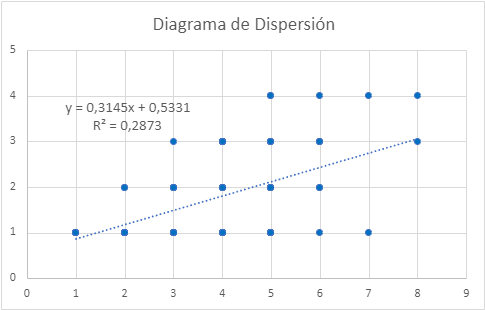
\includegraphics[width=0.6\linewidth]{Imagenes/Ej3.png}
            \caption{Diagrama de dispersión del ejercicio \ref{ej:2.Ejercicio3}}
            \label{fig:ej3:DiagDispersion}
        \end{figure}
    \end{enumerate}
\end{ejercicio}

\begin{ejercicio}\label{ej:2.Ejercicio4}
    Se realiza un estudio sobre la tensión de vapor de agua ($Y$ , en $ml.\;de\;Hg$.) a distintas temperaturas ($X$, en $^\circ C$). Efectuadas 21 medidas, los resultados son:
    \begin{equation*}
        \begin{array}{c||c|ccc|c}
            X\backslash Y & c^x_i & (0.5, 1.5] & (1.5, 2.5] & (2.5, 5.5] & n_{i.}\\ \hline \hline
            c^y_j & & 1 & 2 & 4 \\ \hline
            (1,15] &8& 4 & 2 & 0 & 6\\
            (15, 25] &20& 1 & 4 & 2 & 7\\
            (25,30] &27.5& 0 & 3 & 5 & 8\\ \hline
            n_{.j} &&5 & 9 & 7 & 21
        \end{array}
    \end{equation*}

    Explicar el comportamiento de la tensión de vapor en términos de la temperatura mediante una función lineal. ¿Es adecuado asumir este tipo de relación?\\

    Sea la temperatura, $X$; y la tensión de vapor de agua, $Y$; dos variables estadísticas con población $n=21$ y modalidades $I^x_1, \dots, I^x_3$ e $I^y_1, \dots, I^y_3$ respectivamente, con \emph{distribución de frecuencias}:
        $$\left\{ (I^x_i,I^x_j), n_{ij}\right\}_{\substack{i=1,\dots,3\\j=1,\dots,3}}$$

    En este caso, se pide la recta de regresión de $Y$ sobre $X$. Para ello, calculamos previamente varios datos.
    \begin{equation*}
        \bar{x} = \frac{1}{n}\sum_{i=0}^3 c_i^x n_{i.} = \frac{408}{21} = 19.4286
        \qquad
        \bar{y} = \frac{1}{n}\sum_{j=0}^3 c_j^y n_{.j} = \frac{51}{21} = 2.4286
    \end{equation*}
    \begin{equation*}
        \sigma_x^2 = \frac{1}{n}\sum_{i=0}^3 (c_i^x)^2n_{i.} - \bar{x}^2 = \frac{9234}{21} - \bar{x}^2 = 62.2437
    \end{equation*}
    \begin{equation*}
        \sigma_y^2 = \frac{1}{n}\sum_{j=0}^3 (c_j^y)^2n_{.j} - \bar{y}^2 = \frac{153}{21} - \bar{y}^2 = 1.3876
    \end{equation*}
    \begin{equation*}
        \sigma_{xy} = \frac{1}{n}\sum_{i,j=0}^3 c_i^x c_j^y n_{ij}  -\bar{x}\bar{y} = \frac{1119}{21} -\bar{x}\bar{y} = 6.1014
    \end{equation*}

    La recta de regresión de $Y$ sobre $X$ es:
    \begin{equation*}
        y-\Bar{y} = \frac{\sigma_{xy}}{\sigma_x^2}(x-\Bar{x}) \Longrightarrow y=0.098x +0.5239
    \end{equation*}

    Para ver si asumir este tipo de relación es correcto, vemos el valor del coeficiente de determinación. Haciendo uso de que el ajuste empleado ha sido lineal:
    \begin{equation*}
        \eta_{Y/X}^2 = \frac{\sigma_{ey}^2}{\sigma_y^2} = r^2 = \frac{\sigma_{x,y}^2}{\sigma_x^2 \sigma_y^2} = 0.431
    \end{equation*}

    Como $r^2=0.431$, tenemos que explica solo el $43.1\%$ de los resultados, menos del $50\%$. Por tanto, como dista mucho del $1$, entonces podemos afirmar que en este caso no se ajusta correctamente mediante el ajuste lineal.

    Estos resultados los podemos ver en el diagrama de dispersión de la figura \ref{fig:ej4.DigDisp}.
    \begin{figure}[H]
        \centering
        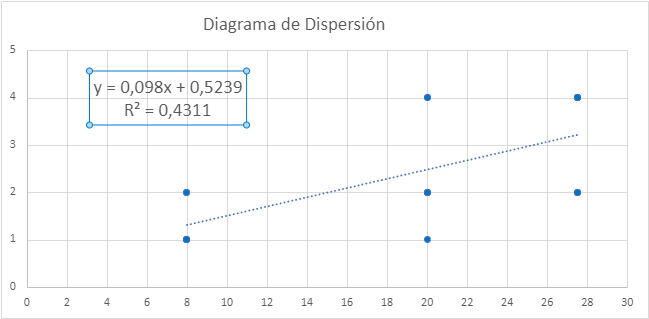
\includegraphics[width=0.6\linewidth]{Imagenes/Ej4.png}
        \caption{Diagrama de dispersión del ejercicio \ref{ej:2.Ejercicio4}}
        \label{fig:ej4.DigDisp}
    \end{figure}
\end{ejercicio}


\begin{ejercicio}
    Estudiar la dependencia o independencia de las variables en cada una de las siguientes distribuciones. Dar, en cada caso, las curvas de regresión y la covarianza de las dos variables.
    \begin{center}
        \hspace{1.3cm}
        Distribución $A$ \hspace{2cm}
        Distribución $B$
    \end{center}
    \begin{equation*}
        \begin{array}{c|ccccc|c}
            X\backslash Y & 1 & 2& 3& 4& 5 &n_{i.}\\ \hline
            10 & 2 & 4 & 6 & 10 & 8 & 30\\
            20 & 1 & 2 & 3 & 5 & 4 & 15\\
            30 & 3 & 6 & 9 & 15 & 12 & 45\\
            40 & 4 & 8 & 12 & 20 & 16 & 60 \\ \hline
            n_{.j} & 10 & 20 & 30 & 50 & 40 & 150
        \end{array}
        \hspace{2cm}
        \begin{array}{c|ccc|c}
            X\backslash Y & 1 & 2 & 3 & n_{i.}\\ \hline
            -1 & 0 & 1 & 0 & 1\\
            0 & 1 & 0 & 1 & 2\\
            1 & 0 & 1 & 0 & 1 \\ \hline
            n_{.j} & 1 & 2 & 1 & 4
        \end{array}
    \end{equation*}

    Sean $X^A$ y $Y^A$ dos variables estadísticas con población $n=150$ y modalidades $x_1^A, \dots, x_4^A$ e $y_1^A, \dots, y_5^A$ respectivamente, con \emph{distribución de frecuencias}:
        $$\left\{ (x_i^A,y_j^A), n_{ij}\right\}_{\substack{i=1,\dots,4\\j=1,\dots,5}}$$

    Por el teorema de la caracterización de la independencia estadística, como $n_{ij}=\frac{n_{i.}n_{.j}}{n} \quad \forall i,j$, tenemos que las variables $X$ e $Y$ son estadísticamente independientes en la distribución $A$. Además, esto también se puede ver, ya que:
    \begin{equation*}
        f_1^j = \frac{1}{5}=f_{1.}
        \qquad
        f_2^j = \frac{1}{10}=f_{2.}
        \qquad
        f_3^j = \frac{3}{10}=f_{3.}
        \qquad
        f_4^j = \frac{2}{5}=f_{4.}
    \end{equation*}
    Como vemos que $f_i^j$ no depende de $j$, tenemos que $X^A$ e $Y^A$ son estadísticamente independientes.

    Sean ahora $X^B$ y $Y^B$ dos variables estadísticas con población $n=4$ y modalidades $x_1^B, \dots, x_3^B$ e $y_1^B, \dots, y_3^B$ respectivamente, con \emph{distribución de frecuencias}:
        $$\left\{ (x_i^B,y_j^B), n_{ij}\right\}_{\substack{i=1,\dots,3\\j=1,\dots,3}}$$

    Como tenemos que $n_{11}=0\neq \frac{1}{4}=\frac{n_{1.}n_{.1}}{n}$, entonces las variables $X,Y$ no son estadísticamente independientes. Tampoco depende $X$ de $Y$ (a $y_2$ le corresponden $x_1$ y $x_3$) ni viceversa (a $x_2$ le corresponden $y_1$ e $y_3$).

    Calculamos ahora las curvas de regresión.
    \begin{enumerate}
        \item \underline{Distribución A}\\
        La covarianza es:
        \begin{equation*}
            \sigma_{xy} = 0,\text{ ya que $X^A$ e $Y^A$ son estadísticamente independientes.}
        \end{equation*}

        Al ser las variables independientes, no tiene sentido calcular la curva de regresión, ya que ninguna de las variables explica la otra.
        
        No obstante, las calculamos. Como son independientes, tenemos que $\bar{x}_j = \bar{x}$, y $\bar{y}_i = \bar{y}$.

        Calculamos las medias aritméticas:
        \begin{equation*}
            \bar{x}=\frac{1}{n} \sum_{i=0}^4 x_in_{i.} = \frac{4350}{150} = 29
            \qquad
            \bar{y}=\frac{1}{n} \sum_{j=0}^5 y_jn_{.j} = \frac{540}{150} = 3.6
        \end{equation*}

        La curva de regresión $X/Y$ pasa por los puntos $(\bar{x}_j, y_j)$. Por tanto, los puntos son:
        \begin{equation*}
            (29, 1) \qquad (29, 2) \qquad (29,3) \qquad (29, 4) \qquad (29, 5)
        \end{equation*}
        La curva de regresión de $X/Y$ la podemos ver en la figura \ref{fig:Ej5.A.1}.
        \begin{figure}[H]
            \centering
            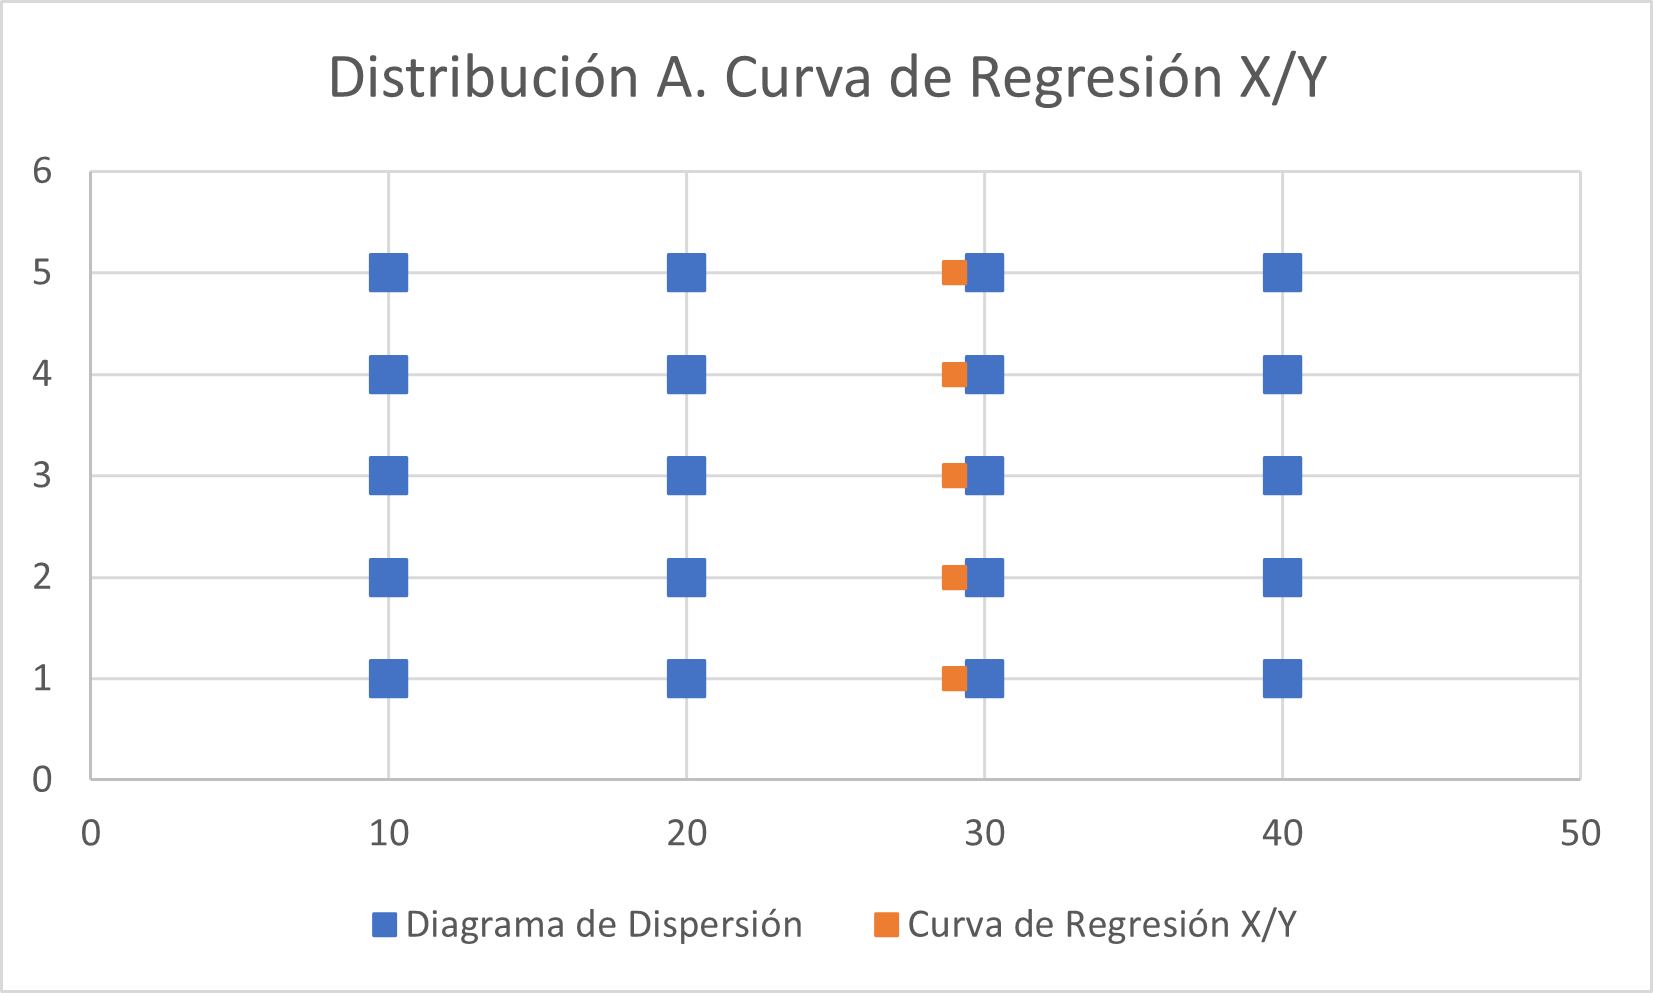
\includegraphics[width=0.7\linewidth]{Imagenes/Ej5.A.1.png}
            \caption{Curva de regresión de tipo I de $X/Y$}
            \label{fig:Ej5.A.1}
        \end{figure}

        La curva de regresión $Y/X$ pasa por los puntos $(x_i, \bar{y}_i)$. Por tanto, los puntos son:
        \begin{equation*}
            (10, 3.6) \qquad (20, 3.6) \qquad (30, 3.6) \qquad (40, 3.6)
        \end{equation*}
        La curva de regresión de $Y/X$ la podemos ver en la figura \ref{fig:Ej5.A.2}.
        \begin{figure}[H]
            \centering
            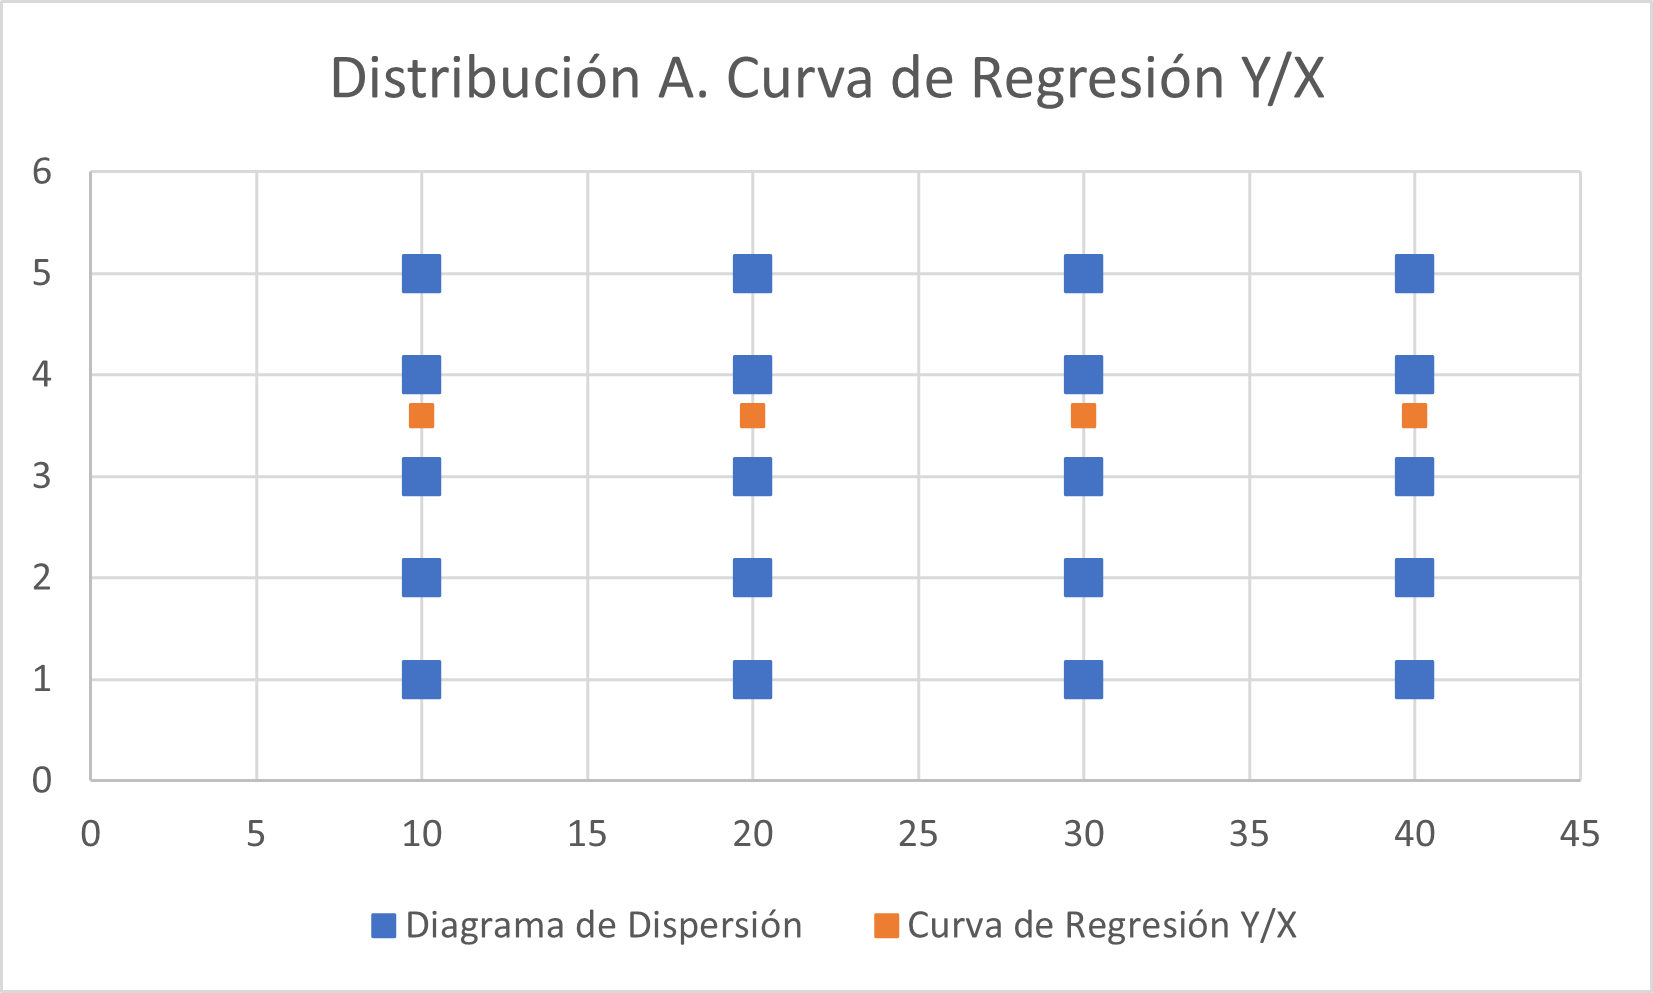
\includegraphics[width=0.7\linewidth]{Imagenes/Ej5.A.2.png}
            \caption{Curva de regresión de tipo I de $Y/X$}
            \label{fig:Ej5.A.2}
        \end{figure}

        Como podemos ver, al ser las variables independientes, la curva de regresión no aporta información relevante. Los puntos se sitúan paralelos a los ejes a la altura de la media que se quiere explicar.        


        \item \underline{Distribución B}\\
        La covarianza es:        
        \begin{equation*}
            \sigma_{xy} = \frac{1}{n} \sum_{i,j=1}^3 x_i y_j n_{ij} -\bar{x}\bar{y} = \frac{0}{4} - 0 = 0
        \end{equation*}

        Por tanto, aquí podemos ver que si las variables son independientes, entonces su covarianza es nula, pero que el recíproco no es cierto. Ejemplo de lo segundo es esto.

        Calculamos ahora la curva de regresión de tipo I de $Y/X$, que pasa por los puntos $(x_i, \bar{y}_i)$:
        \begin{equation*}
            \bar{y}_1 = \frac{1}{n_{1.}}\sum_{j=1}^3 y_jn_{1j} = \frac{2}{1} = 2
            \quad
            \bar{y}_2 = \frac{1}{n_{2.}}\sum_{j=1}^3 y_jn_{2j} = \frac{4}{2} = 2
        \end{equation*}
        \begin{equation*}
            \bar{y}_3 = \frac{1}{n_{3.}}\sum_{j=1}^3 y_jn_{3j} = \frac{2}{1} = 2
        \end{equation*}

        Por tanto, los puntos son:
        \begin{equation*}
            (-1, 2) \qquad (0, 2) \qquad (1, 2)
        \end{equation*}
        
        La curva de regresión de $Y/X$ la podemos ver en la figura \ref{fig:Ej5.B.1}.
        \begin{figure}[H]
            \centering
            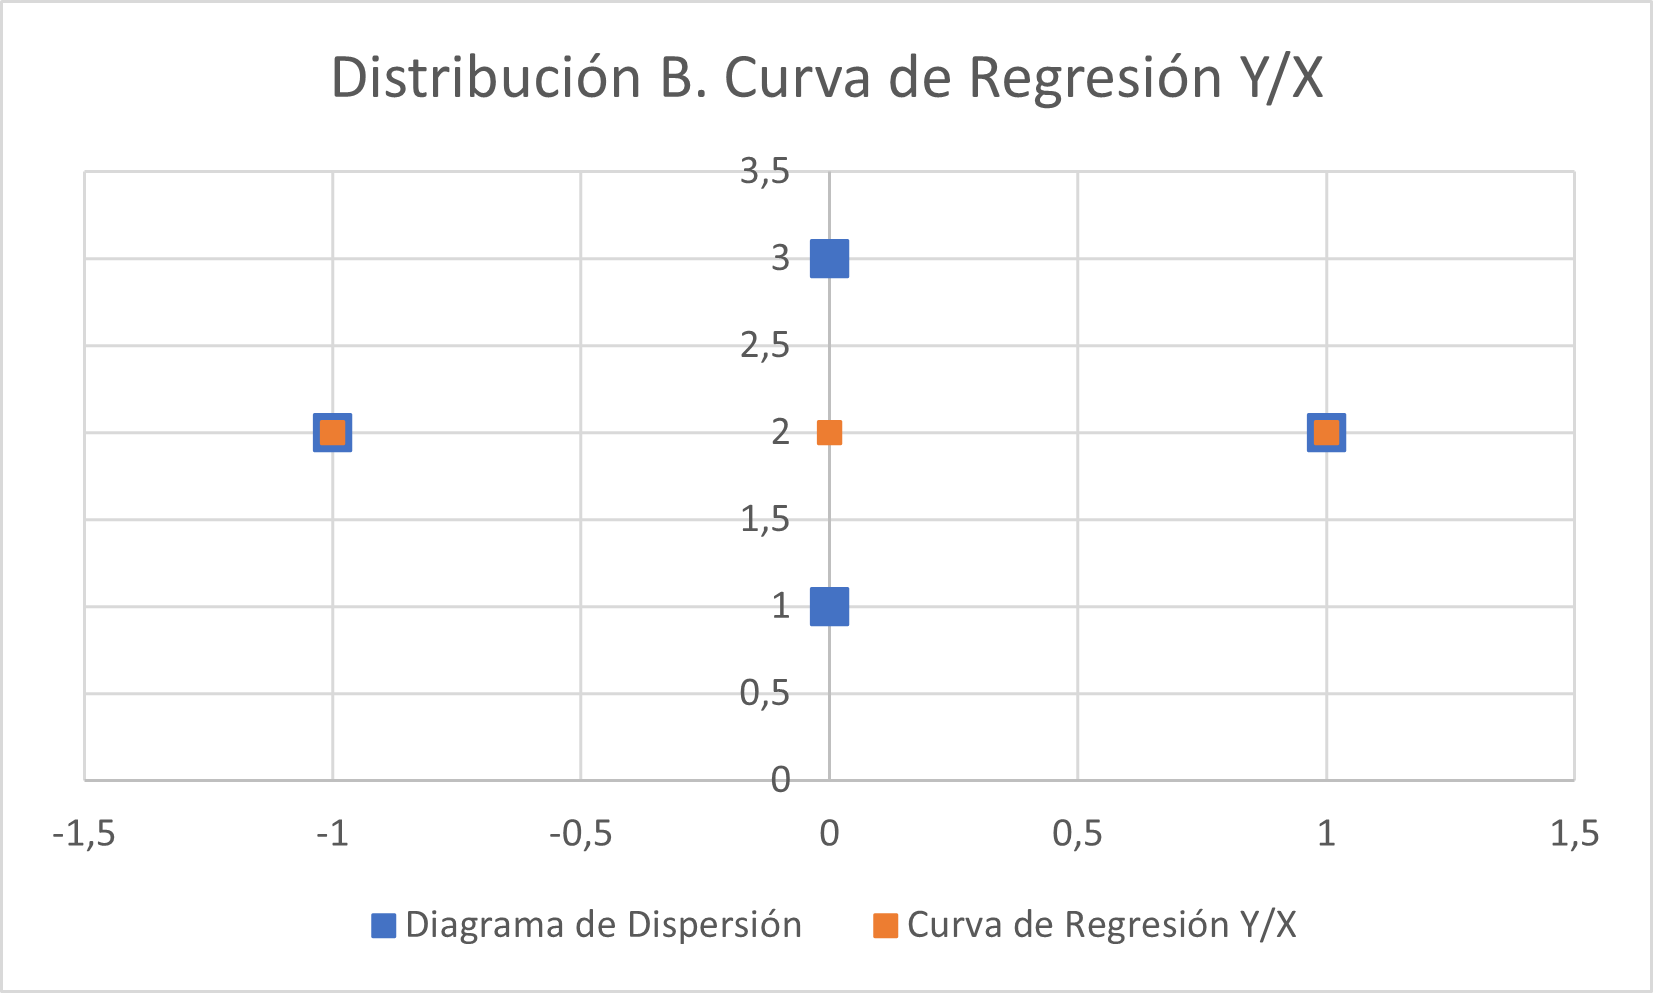
\includegraphics[width=0.7\linewidth]{Imagenes/Ej5.B.1.png}
            \caption{Curva de regresión de tipo I de $Y/X$}
            \label{fig:Ej5.B.1}
        \end{figure}

        Calculamos ahora la curva de regresión de tipo I de $X/Y$, que pasa por los puntos $(\bar{x}_j, y_j)$:
        \begin{equation*}
            \bar{x}_1 = \frac{1}{n_{.1}}\sum_{i=1}^3 x_in_{i1} = \frac{0}{1} = 0
            \quad
            \bar{x}_2 = \frac{1}{n_{.2}}\sum_{i=1}^3 x_in_{i2} = \frac{0}{2} = 0
        \end{equation*}
        \begin{equation*}
            \bar{x}_3 = \frac{1}{n_{.3}}\sum_{i=1}^3 x_in_{i3} = \frac{0}{1} = 0
        \end{equation*}

        Por tanto, los puntos son:
        \begin{equation*}
            (0,1) \qquad (0, 2) \qquad (0,3)
        \end{equation*}

        La curva de regresión de $X/Y$ la podemos ver en la figura \ref{fig:Ej5.B.2}.
        \begin{figure}[H]
            \centering
            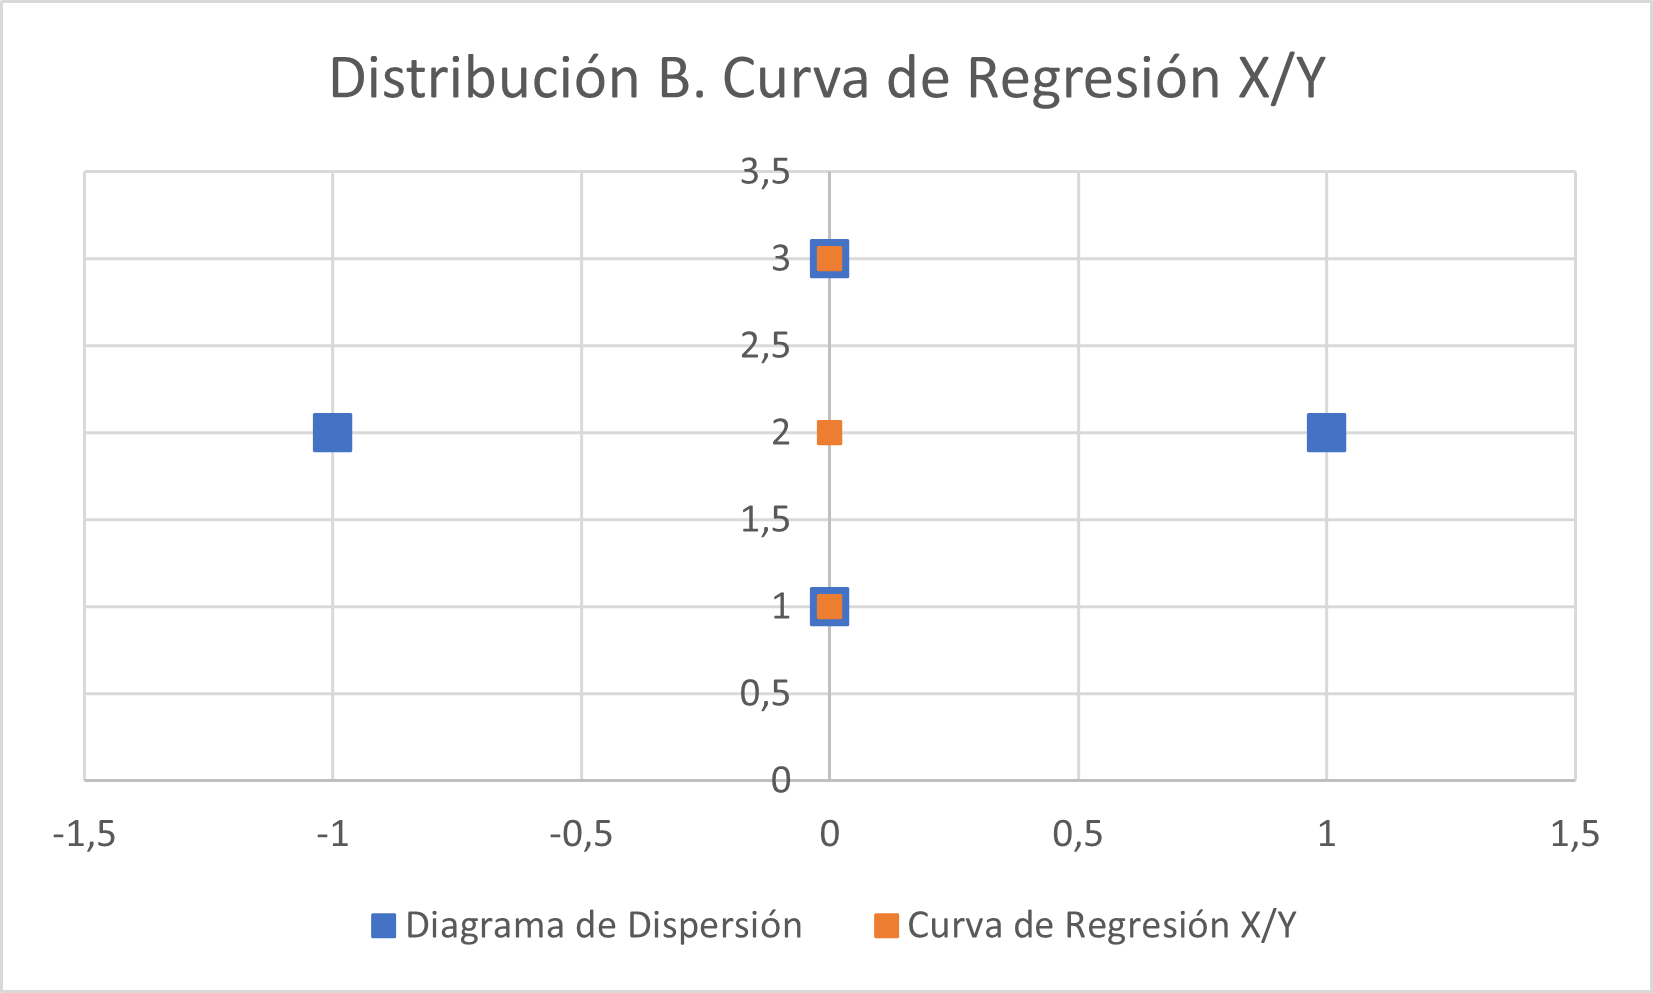
\includegraphics[width=0.7\linewidth]{Imagenes/Ej5.B.2.png}
            \caption{Curva de regresión de tipo I de $X/Y$}
            \label{fig:Ej5.B.2}
        \end{figure}
    \end{enumerate}
    
\end{ejercicio}

\begin{ejercicio}
    Dada la siguiente distribución bidimensional:
    \begin{equation*}
        \begin{array}{c|cccc|c}
            X\backslash Y & 1 & 2& 3& 4 & n_{i.}\\ \hline
            10 & 1 & 3 & 0 & 0 & 4\\
            12 & 0 & 1 & 4 & 3 & 8\\
            14 & 2 & 0 & 0 & 2 & 4\\
            16 & 4 & 0 & 0 & 0 & 4\\ \hline
            n_{.j} & 7 & 4 & 4 & 5 & 20
        \end{array}
    \end{equation*}

    \begin{enumerate}
        \item ¿Son estadísticamente independientes $X$ e $Y$?
        
        Sean $X$ y $Y$ dos variables estadísticas con población $n=20$ y modalidades $x_1, \dots, x_4$ e $y_1, \dots, y_4$ respectivamente, con \emph{distribución de frecuencias}:
        $$\left\{ (x_i,y_j), n_{ij}\right\}_{\substack{i=1,\dots,4\\j=1,\dots,4}}$$

        Veamos ahora si son independientes:
        \begin{equation*}
            f_1^1 = \frac{n_{11}}{n_{.1}} = \frac{1}{7} \qquad f_{1.} = \frac{n_{1.}}{n} = \frac{4}{20}
        \end{equation*}
        Como $f_1^1\neq f_{1.} \Longrightarrow $ $X$ y $Y$ por lo que no son independientes.
        
        \item Calcular y representar las curvas de regresión de $X/Y$ e $Y/X$.

        Calculo en primer lugar la curva de regresión de $X/Y$. Esto son los puntos $(\bar{x}_j, y_j)\;\forall j=1,\dots,4$.
        \begin{equation*}
            \bar{x_1} = \frac{1}{n_{\cdot1}}\sum_{i=0}^n x_in_{i1} = \frac{102}{7} = 14.5715
            \qquad
            \bar{x_2} = \frac{1}{n_{\cdot2}}\sum_{i=0}^n x_in_{i2} = \frac{42}{4} = 10.5
        \end{equation*}
        \begin{equation*}
            \bar{x_3} = \frac{1}{n_{\cdot3}}\sum_{i=0}^n x_in_{i3} = \frac{48}{4} = 12
            \qquad
            \bar{x_4} = \frac{1}{n_{\cdot4}}\sum_{i=0}^n x_in_{i4} = \frac{64}{5} = 12.8
        \end{equation*}
        Por tanto, la curva de regresión de tipo I de $X/Y$ es la que pasa por los puntos:
        \begin{equation*}
            (14.5715,\;1)\qquad (10.5,\;2) \qquad (12,\;3) \qquad (12.8,\;4)
        \end{equation*}
        
        Su representación se encuentra en la figura \ref{fig:Ej6.b.1}.
        \begin{figure}[H]
            \centering
            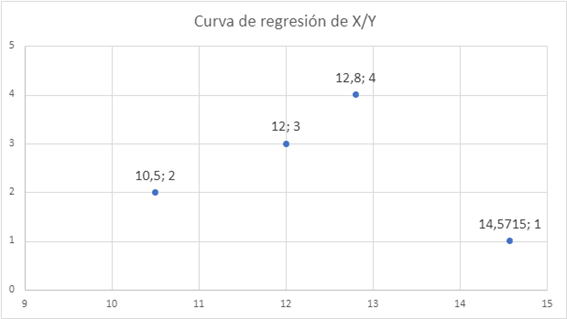
\includegraphics[width=0.6\linewidth]{Imagenes/Ej6.b.1.png}
            \caption{Curva de regresión de tipo I de $X$/$Y$}
            \label{fig:Ej6.b.1}
        \end{figure}

        Calculo ahora la curva de regresión de $Y/X$. Esto son los puntos $(x_i, \bar{y}_i)\;\forall i=1,\dots,4$.
        \begin{equation*}
            \bar{y_1} = \frac{1}{n_{1.}}\sum_{j=0}^n y_jn_{1j} = \frac{7}{4} = 1.75
            \qquad
            \bar{y_2} = \frac{1}{n_{2.}}\sum_{j=0}^n y_jn_{2j} = \frac{26}{8} = 3.25
        \end{equation*}
        \begin{equation*}
            \bar{y_3} = \frac{1}{n_{3.}}\sum_{j=0}^n y_jn_{3j} = \frac{10}{4} = 2.5
            \qquad
            \bar{y_4} = \frac{1}{n_{4.}}\sum_{j=0}^n y_jn_{4j} = \frac{4}{4} = 1
        \end{equation*}
        Por tanto, la curva de regresión de tipo I de $Y/X$ es la que pasa por los puntos:
        \begin{equation*}
            (10,\;1.75)\qquad (12,\;3.25) \qquad (14,\;2.5) \qquad (16,\;1)
        \end{equation*}
        
        Su representación se encuentra en la figura \ref{fig:Ej6.b.2}.
        \begin{figure}[H]
            \centering
            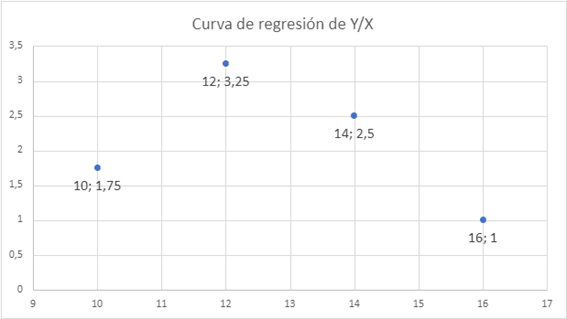
\includegraphics[width=0.6\linewidth]{Imagenes/Ej6.b.2.png}
            \caption{Curva de regresión de tipo I de $Y$/$X$}
            \label{fig:Ej6.b.2}
        \end{figure}

        \item Cuantificar el grado en que cada variable es explicada por la otra mediante la correspondiente curva de regresión.

        En primer lugar, calculo la varianza explicada por cada curva de regresión. Para ello, necesito previamente las medias aritméticas.
        \begin{equation*}
            \bar{x} = \frac{1}{n} \sum_{i=0}^4x_i n_{i.} = \frac{256}{20} = 12.8
            \qquad
            \bar{y} = \frac{1}{n} \sum_{j=0}^4 y_j n_{.j} = \frac{47}{20} = 2.35
        \end{equation*}
        \begin{equation*}
            \sigma_{ey}^2 = \frac{1}{n}\sum_{i,j=1}^4 n_{ij}(\hat{y}_j-\bar{y})^2
            = \frac{1}{n}\sum_{i,j=1}^4 n_{ij}(\bar{y}_i-\bar{y})^2 
            = \frac{1}{n}\sum_{i=1}^4 n_{i.}(\bar{y}_i-\bar{y})^2 =\frac{15.3}{20} = 0.765
        \end{equation*}
        \begin{equation*}
            \sigma_{ex}^2 = \frac{1}{n}\sum_{i,j=1}^4 n_{ij}(\hat{x}_i-\bar{x})^2
            = \frac{1}{n}\sum_{i,j=1}^4 n_{ij}(\bar{x}_j-\bar{x})^2 
            = \frac{1}{n}\sum_{j=1}^4 n_{.j}(\bar{x}_j-\bar{x})^2 =\frac{45.6875}{20} = 2.2845
        \end{equation*}

        Para poder comparar, necesito el coeficiente de determinación. Para ello, calculo también las varianzas de cada variable.
        \begin{equation*}
            \sigma_x^2 = \frac{1}{n}\sum_{i=0}^4 n_{i.}x_i^2 - \bar{x}^2 = \frac{3360}{20} - \bar{x}^2 = 4.16
        \end{equation*}
        \begin{equation*}
            \sigma_y^2 = \frac{1}{n}\sum_{j=0}^4 n_{.j}y_j^2 - \bar{y}^2 = \frac{139}{20} - \bar{y}^2 = 1.4275
        \end{equation*}

        Por tanto, los coeficientes de determinación son:
        \begin{equation*}
            \eta_{X/Y}^2 = \frac{\sigma_{ex}^2}{\sigma_x^2} = 0.5492
            \qquad
            \eta_{Y/X}^2 = \frac{\sigma_{ey}^2}{\sigma_y^2} = 0.5359
        \end{equation*}

        Como podemos ver, la curva de regresión de $X/Y$ tiene un coeficiente de determinación menor, por lo que la variable $X$ es mejor explicada por la variable $Y$ que al revés.

        \item ¿Están $X$ e $Y$ correlacionadas linealmente? Dar las expresiones de las rectas de regresión.\\

        Para calcular el coeficiente de determinación, necesito previamente la covarianza.
        \begin{equation*}
            \sigma_{xy} = \frac{1}{n}\sum_{i,j=0}^4 n_{ij}x_iy_j - \bar{x}\bar{y} = \frac{586}{20}- \bar{x}\bar{y} = -0.78
        \end{equation*}

        Por tanto, la recta de regresión de $Y$ sobre $X$ es:
        \begin{equation*}
            y-\bar{y} = \frac{\sigma_{xy}}{\sigma_x^2}(x-\bar{x}) \Longrightarrow y=-0.188x+4.75
        \end{equation*}

        La recta de regresión de $X$ sobre $Y$ es:
        \begin{equation*}
            x-\bar{x} = \frac{\sigma_{xy}}{\sigma_y^2}(y-\bar{y}) \Longrightarrow x=-0.546y+14.083
        \end{equation*}

        Para ver si están correlacionadas linealmente, calculo el coeficiente de correlación lineal:
        \begin{equation*}
            r = \frac{\sigma_{xy}}{\sigma_x \sigma_y} = -0.32008
        \end{equation*}

        Como el valor de $r$ no se acerca ni a $+1$ ni a $-1$, concluimos que el nivel de correlación entre ambas variables es bajo.
    \end{enumerate}
\end{ejercicio}

\begin{ejercicio}
    Para cada una de las distribuciones:
    \begin{center}
        Distribución $A$ \hspace{1.8cm}
        Distribución $B$ \hspace{1.9cm}
        Distribución $C$
    \end{center}
    \begin{equation*}
        \begin{array}{c|ccc}
            X\backslash Y & 10 & 15 & 20\\ \hline
            1 & 0 & 2 & 0\\
            2 & 1 & 0 & 0\\
            3 & 0 & 0 & 3\\
            4 & 0 & 1 & 0 
        \end{array}
        \qquad
        \begin{array}{c|ccc}
            X\backslash Y & 10 & 15 & 20\\ \hline
            1 & 0 & 2 & 0\\
            2 & 1 & 0 & 0\\
            3 & 0 & 0 & 3\\
        \end{array}
        \qquad
        \begin{array}{c|cccc}
            X\backslash Y & 10 & 15 & 20 & 25\\ \hline
            1 & 0 & 3 & 0 & 1\\
            2 & 0 & 0 & 1 & 0\\
            3 & 2 & 0 & 0 & 0\\
        \end{array}
    \end{equation*}
    \begin{enumerate}
        \item ¿Dependen funcionalmente $X$ de $Y$ o $Y$ de $X$?\\

        Sean $X^A$ y $Y^A$ dos variables estadísticas con población $n=7$ y modalidades $x_1^A, \dots, x_4^A$ e $y_1^A, \dots, y_3^A$ respectivamente, con \emph{distribución de frecuencias}:
        $$\left\{ (x_i^A,y_j^A), n_{ij}\right\}_{\substack{i=1,\dots,4\\j=1,\dots,3}}$$
        
        En el caso de la distribución $A$, la variable $Y^A$ depende funcionalmente de la variable $X^A$, ya que a cada modalidad de $X^A$ le corresponde una única modalidad de $Y^A$ con frecuencia no nula.

        No obstante, la variable $X^A$ no depende funcionalmente de $Y^A$, ya que a la modalidad $y_2^A$ le corresponden dos modalidades con frecuencias no nulas, $x^A_1$ y $x^A_4$.

        Sean ahora $X^B$ y $Y^B$ dos variables estadísticas con población $n=6$ y modalidades $x_1^B, \dots, x_3^B$ e $y_1^B, \dots, y_3^B$ respectivamente, con \emph{distribución de frecuencias}:
        $$\left\{ (x_i^B,y_j^B), n_{ij}\right\}_{\substack{i=1,\dots,3\\j=1,\dots,3}}$$

        En el caso de la distribución $B$, la dependencia lineal es recíproca, ya que a cada modalidad de cada una de las variables le corresponde una única modalidad de la otra variable con frecuencia no nula.

        Sean por último $X^C$ y $Y^C$ dos variables estadísticas con población $n=7$ y modalidades $x_1^C, \dots, x_3^C$ e $y_1^C, \dots, y_4^C$ respectivamente, con \emph{distribución de frecuencias}:
        $$\left\{ (x_i^C,y_j^C), n_{ij}\right\}_{\substack{i=1,\dots,3\\j=1,\dots,4}}$$

        En el caso de la distribución $C$, la variable $X^C$ depende funcionalmente de la variable $Y^C$, ya que a cada modalidad de $Y^C$ le corresponde una única modalidad de $X^C$ con frecuencia no nula.

        No obstante, la variable $Y^C$ no depende funcionalmente de $X^C$, ya que a la modalidad $x_1^C$ le corresponden dos modalidades con frecuencias no nulas, $y^C_2$ y $y^C_4$.
        
        \item Calcular las curvas de regresión y comentar los resultados.
        \begin{enumerate}
            \item Distribución A\\
            La curva de regresión de tipo I de $X/Y$ (ver figura \ref{fig:Ej7.2.A.1}) pasa por los puntos $(\bar{x}_j, y_j)$:
            \begin{equation*}
                \bar{x}_1 = \frac{1}{n_{.1}}\sum_{i=0}^4 x_i^A n_{i1} = \frac{2}{1} = 2
                \qquad
                \bar{x}_2 = \frac{1}{n_{.2}}\sum_{i=0}^4 x_i^A n_{i2} = \frac{6}{3} = 2
            \end{equation*}
            \begin{equation*}
                \bar{x}_3 = \frac{1}{n_{.3}}\sum_{i=0}^4 x_i^A n_{i3} = \frac{9}{3} = 3
            \end{equation*}

            Los puntos son:
            \begin{equation*}
                (2,10)\qquad (2,15) \qquad (3,20)
            \end{equation*}
            \begin{figure}[H]
                \centering
                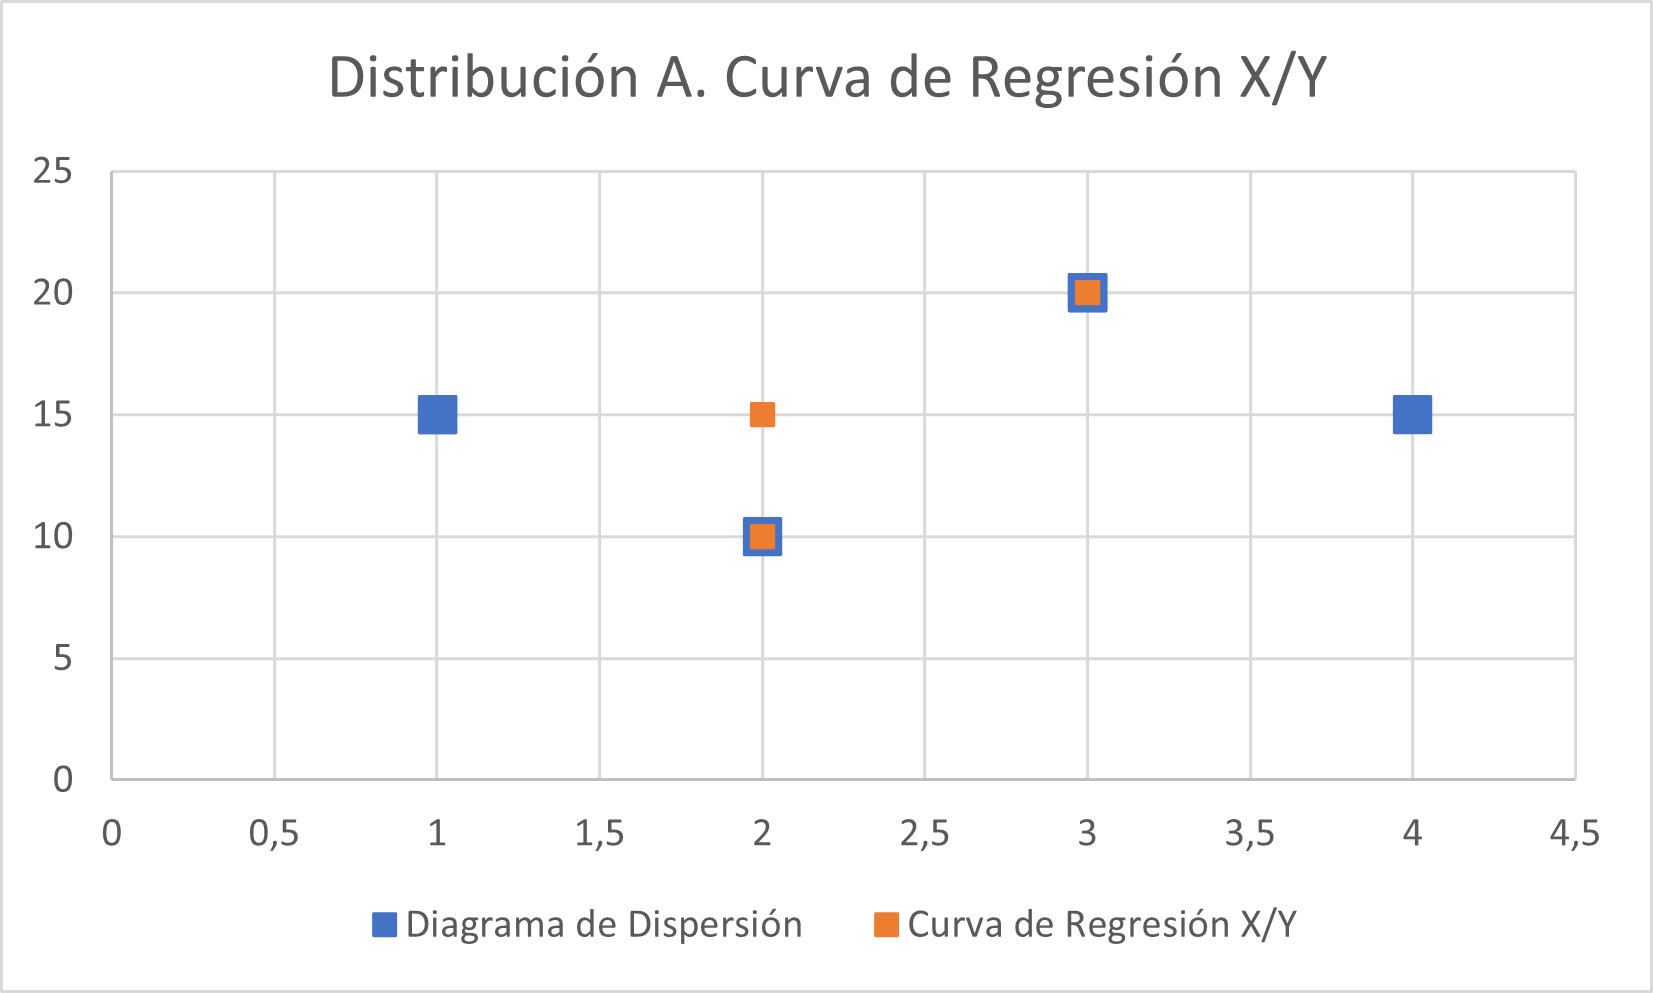
\includegraphics[width=0.6\linewidth]{Imagenes/Ej7.2.A.1.png}
                \caption{Curva de Regresión $X/Y$ de la distribución A.}
                \label{fig:Ej7.2.A.1}
            \end{figure}
            

            La curva de regresión de tipo I de $Y/X$ (ver figura \ref{fig:Ej7.2.A.2}) pasa por los puntos $(x_i, \bar{y}_i)$:
            \begin{equation*}
                \bar{y}_1 = \frac{1}{n_{1.}}\sum_{j=0}^3 y_j^A n_{1j} = \frac{30}{2} = 15
                \qquad
                \bar{y}_2 = \frac{1}{n_{2.}}\sum_{j=0}^3 y_j^A n_{2j} = \frac{10}{1} = 10
            \end{equation*}
            \begin{equation*}
                \bar{y}_3 = \frac{1}{n_{3.}}\sum_{j=0}^3 y_j^A n_{3j} = \frac{60}{3} = 20
                \qquad
                \bar{y}_4 = \frac{1}{n_{4.}}\sum_{j=0}^3 y_j^A n_{4j} = \frac{15}{1} = 15
            \end{equation*}

            Los puntos son:
            \begin{equation*}
                (1,15)\qquad (2,10) \qquad (3,20) \qquad (4,15)
            \end{equation*}
            \begin{figure}[H]
                \centering
                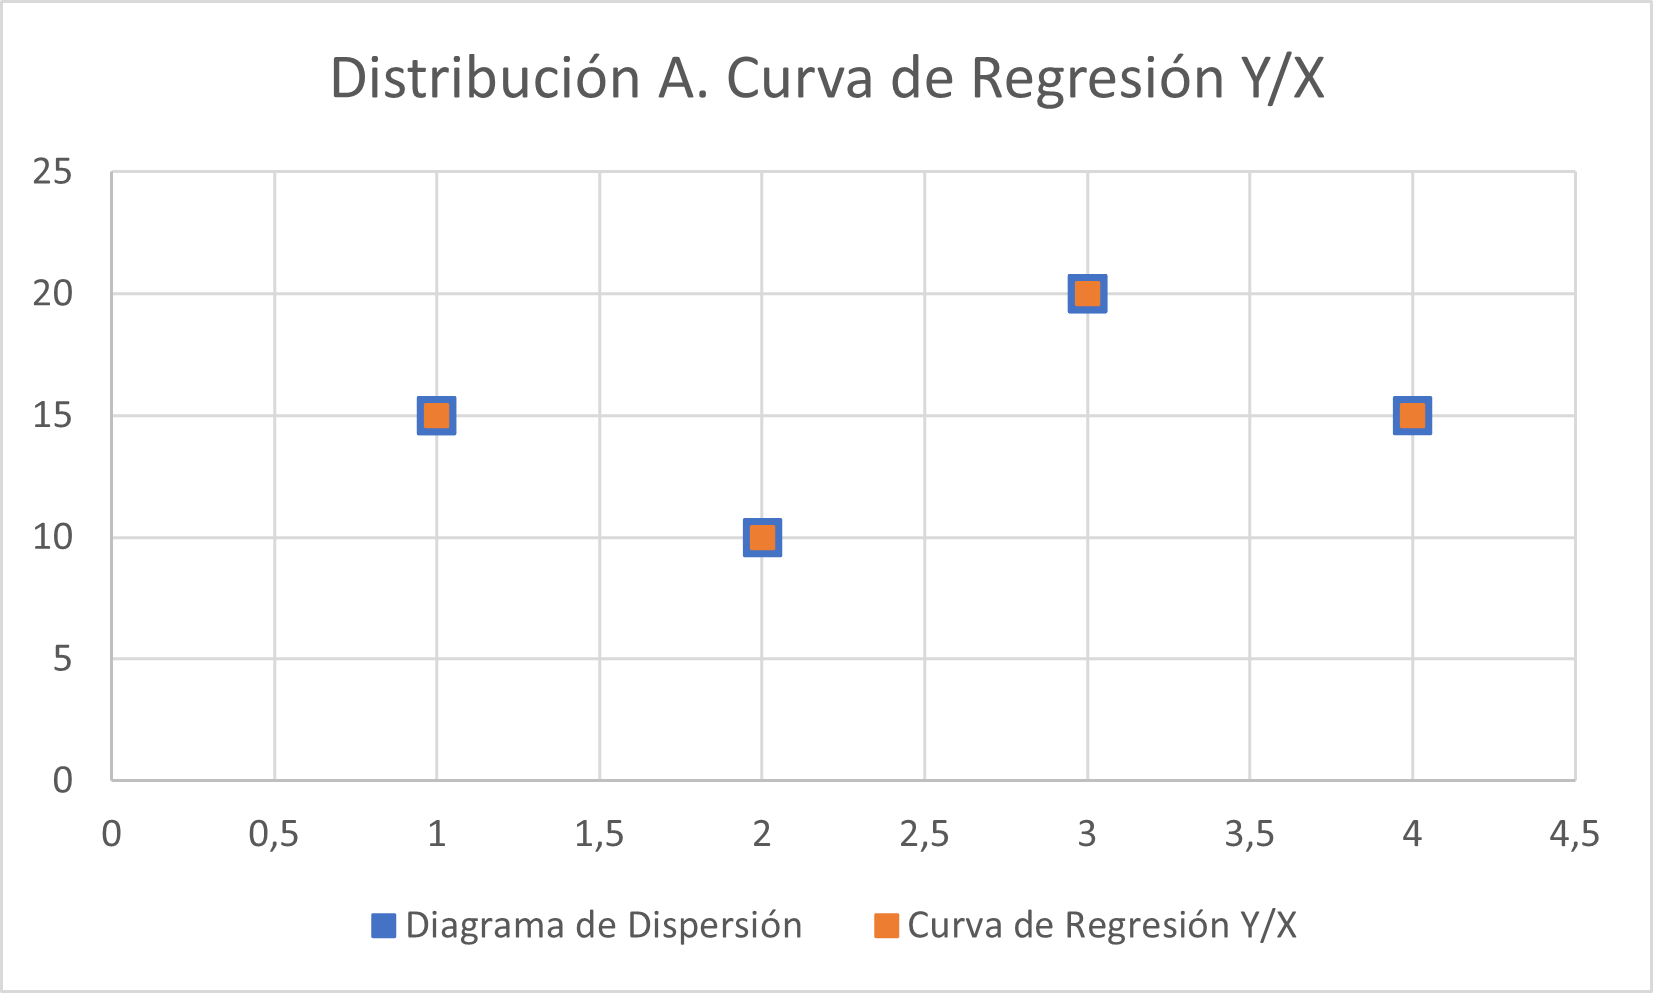
\includegraphics[width=0.6\linewidth]{Imagenes/Ej7.2.A.2.png}
                \caption{Curva de Regresión $Y/X$ de la distribución A.}
                \label{fig:Ej7.2.A.2}
            \end{figure}
            
            \item Distribución B\\

            La curva de regresión de tipo I de $X/Y$ (ver figura \ref{fig:Ej7.2.B.1}) pasa por los puntos $(\bar{x}_j, y_j)$:
            \begin{equation*}
                \bar{x}_1 = \frac{1}{n_{.1}}\sum_{i=0}^3 x_i^B n_{i1} = \frac{2}{1} = 2
                \qquad
                \bar{x}_2 = \frac{1}{n_{.2}}\sum_{i=0}^3 x_i^B n_{i2} = \frac{2}{2} = 1
            \end{equation*}
            \begin{equation*}
                \bar{x}_3 = \frac{1}{n_{.3}}\sum_{i=0}^3 x_i^B n_{i3} = \frac{9}{3} = 3
            \end{equation*}

            Los puntos son:
            \begin{equation*}
                (2,10)\qquad (1,15) \qquad (3,20)
            \end{equation*}
            \begin{figure}[H]
                \centering
                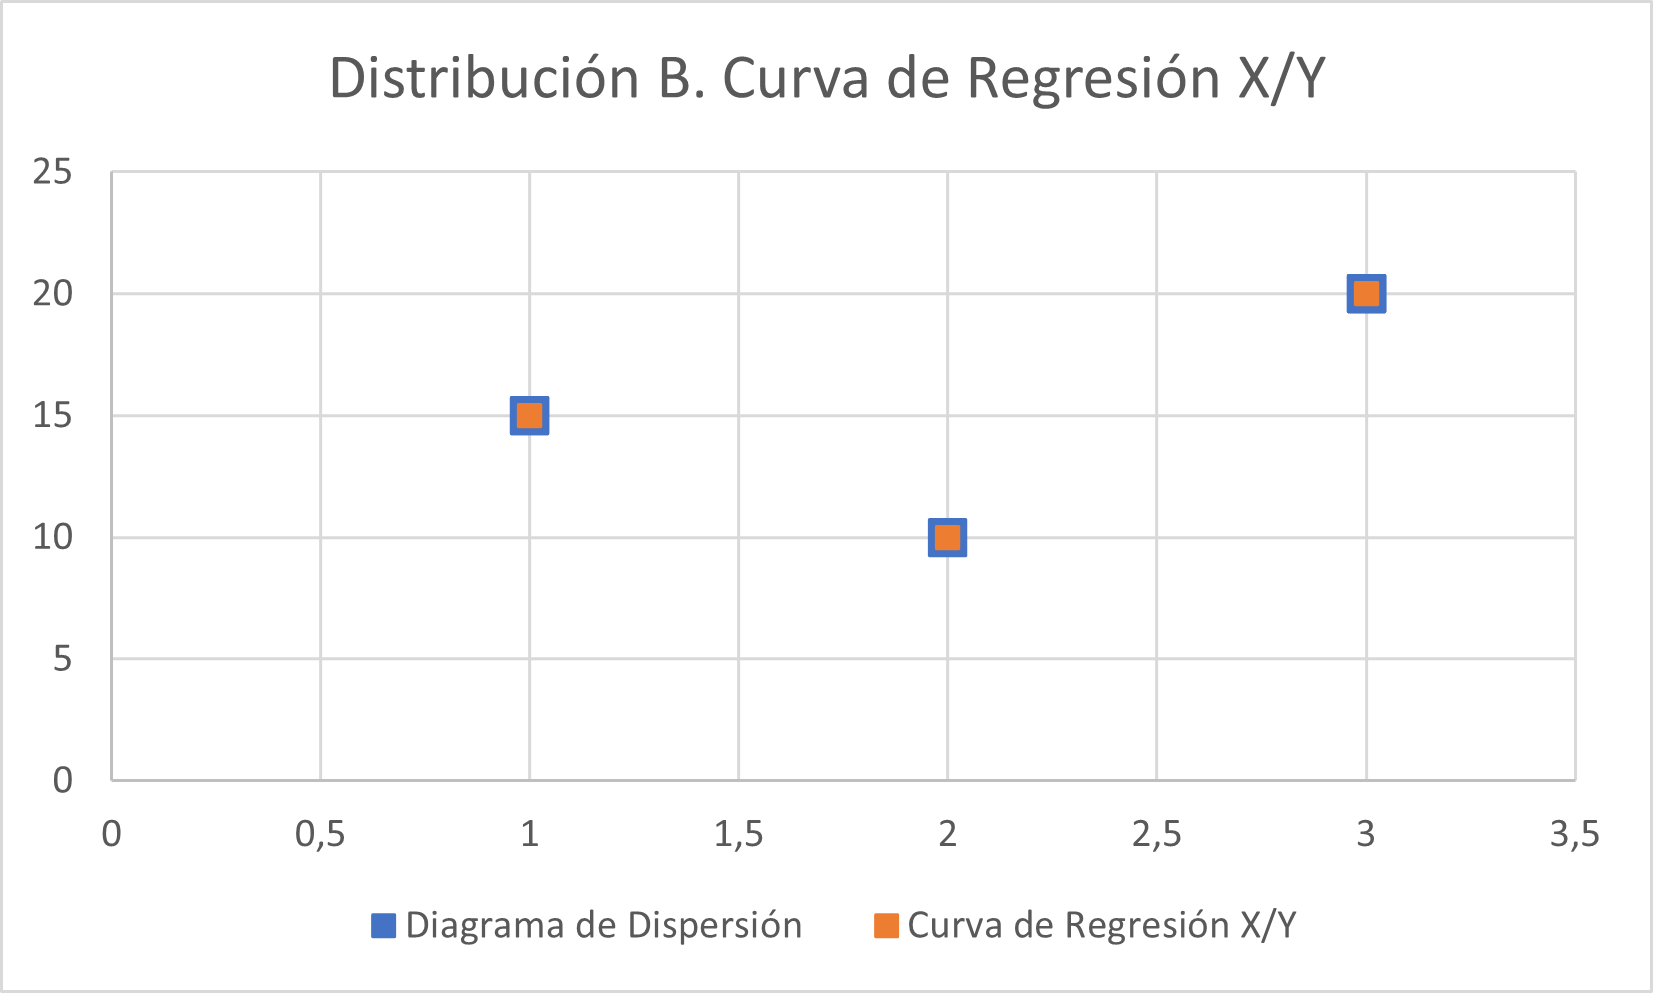
\includegraphics[width=0.6\linewidth]{Imagenes/Ej7.2.B.1.png}
                \caption{Curva de Regresión $X/Y$ de la distribución B.}
                \label{fig:Ej7.2.B.1}
            \end{figure}
            

            La curva de regresión de tipo I de $Y/X$ (ver figura \ref{fig:Ej7.2.B.2}) pasa por los puntos $(x_i, \bar{y}_i)$:
            \begin{equation*}
                \bar{y}_1 = \frac{1}{n_{1.}}\sum_{j=0}^3 y_j^B n_{1j} = \frac{30}{2} = 15
                \qquad
                \bar{y}_2 = \frac{1}{n_{2.}}\sum_{j=0}^3 y_j^B n_{2j} = \frac{10}{1} = 10
            \end{equation*}
            \begin{equation*}
                \bar{y}_3 = \frac{1}{n_{3.}}\sum_{j=0}^3 y_j^B n_{3j} = \frac{60}{3} = 20
            \end{equation*}

            Los puntos son:
            \begin{equation*}
                (1,15)\qquad (2,10) \qquad (3,20)
            \end{equation*}
            \begin{figure}[H]
                \centering
                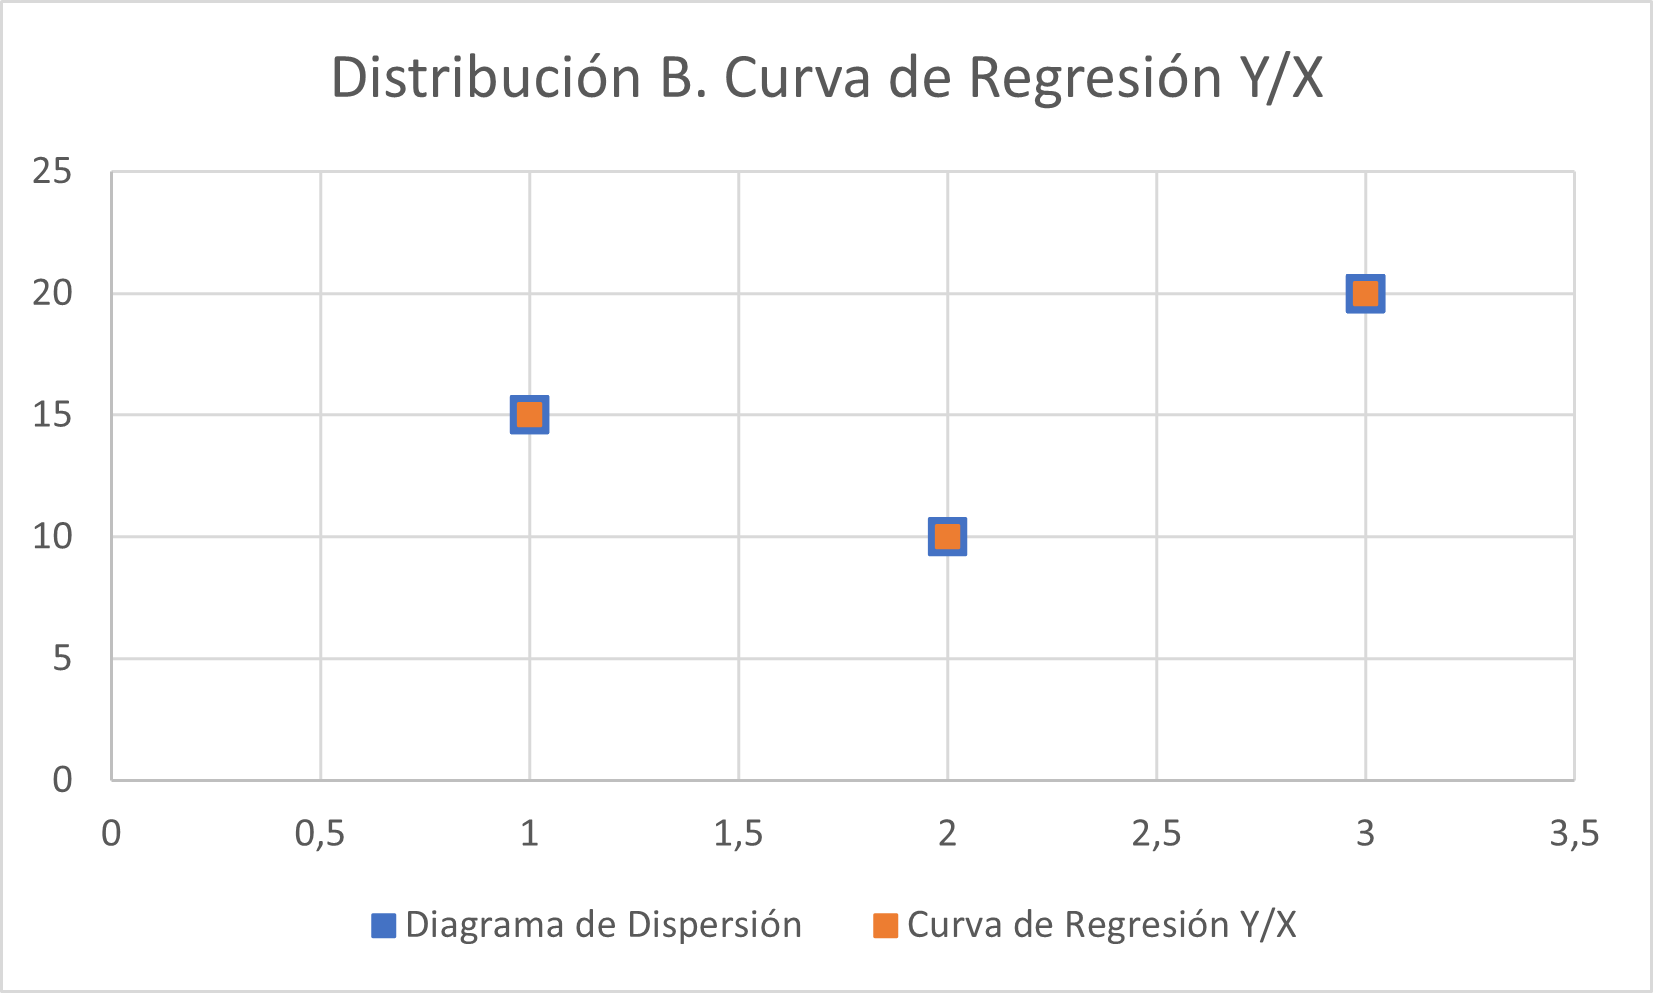
\includegraphics[width=0.6\linewidth]{Imagenes/Ej7.2.B.2.png}
                \caption{Curva de Regresión $Y/X$ de la distribución B.}
                \label{fig:Ej7.2.B.2}
            \end{figure}
            
            \item Distribución C\\
            La curva de regresión de tipo I de $X/Y$ (ver figura \ref{fig:Ej7.2.C.1}) pasa por los puntos $(\bar{x}_j, y_j)$:
            \begin{equation*}
                \bar{x}_1 = \frac{1}{n_{.1}}\sum_{i=0}^3 x_i^C n_{i1} = \frac{6}{2} = 3
                \qquad
                \bar{x}_2 = \frac{1}{n_{.2}}\sum_{i=0}^3 x_i^C n_{i2} = \frac{3}{3} = 1
            \end{equation*}
            \begin{equation*}
                \bar{x}_3 = \frac{1}{n_{.3}}\sum_{i=0}^3 x_i^C n_{i3} = \frac{2}{1} = 2
                \qquad
                \bar{x}_4 = \frac{1}{n_{.4}}\sum_{i=0}^3 x_i^C n_{i4} = \frac{1}{1} = 1
            \end{equation*}

            Los puntos son:
            \begin{equation*}
                (3,10)\qquad (1,15) \qquad (2,20) \qquad (1,25)
            \end{equation*}
            \begin{figure}[H]
                \centering
                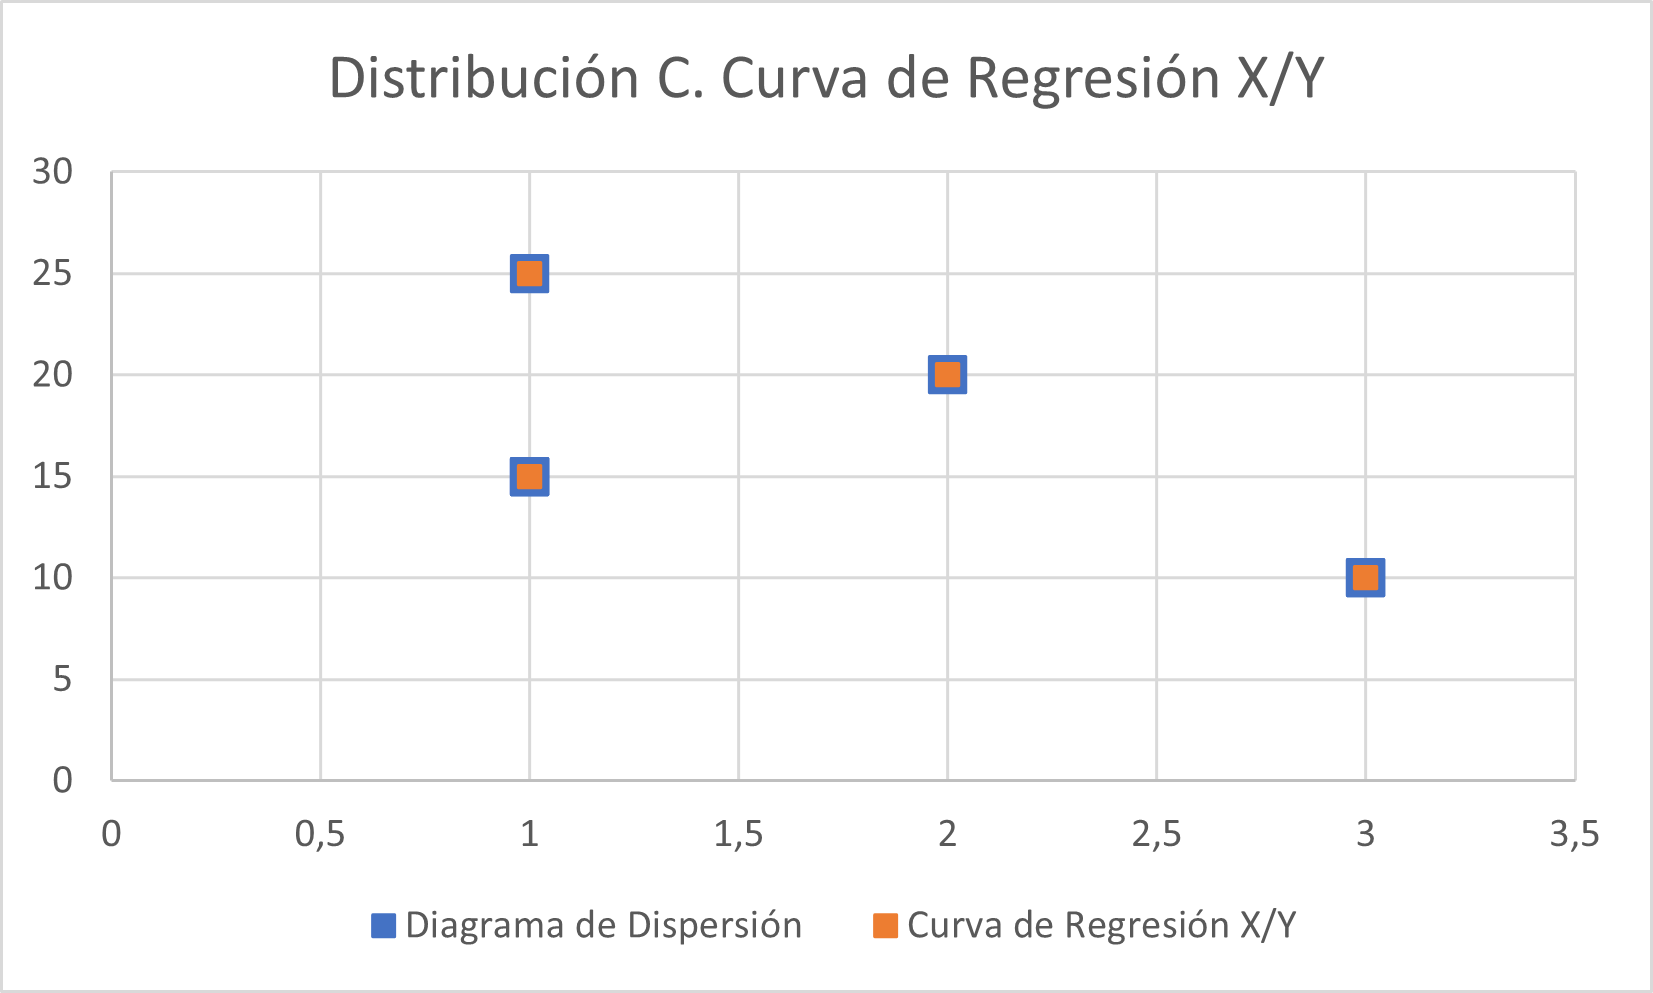
\includegraphics[width=0.6\linewidth]{Imagenes/Ej7.2.C.1.png}
                \caption{Curva de Regresión $X/Y$ de la distribución C.}
                \label{fig:Ej7.2.C.1}
            \end{figure}
            

            La curva de regresión de tipo I de $Y/X$ (ver figura \ref{fig:Ej7.2.C.2}) pasa por los puntos $(x_i, \bar{y}_i)$:
            \begin{equation*}
                \bar{y}_1 = \frac{1}{n_{1.}}\sum_{j=0}^4 y_j^C n_{1j} = \frac{55}{4} = 17.5
                \qquad
                \bar{y}_2 = \frac{1}{n_{2.}}\sum_{j=0}^4 y_j^C n_{2j} = \frac{20}{1} = 20
            \end{equation*}
            \begin{equation*}
                \bar{y}_3 = \frac{1}{n_{3.}}\sum_{j=0}^4 y_j^C n_{3j} = \frac{20}{2} = 10
            \end{equation*}

            Los puntos son:
            \begin{equation*}
                (1,\;17.5)\qquad (2,20) \qquad (3,10)
            \end{equation*}
            \begin{figure}[H]
                \centering
                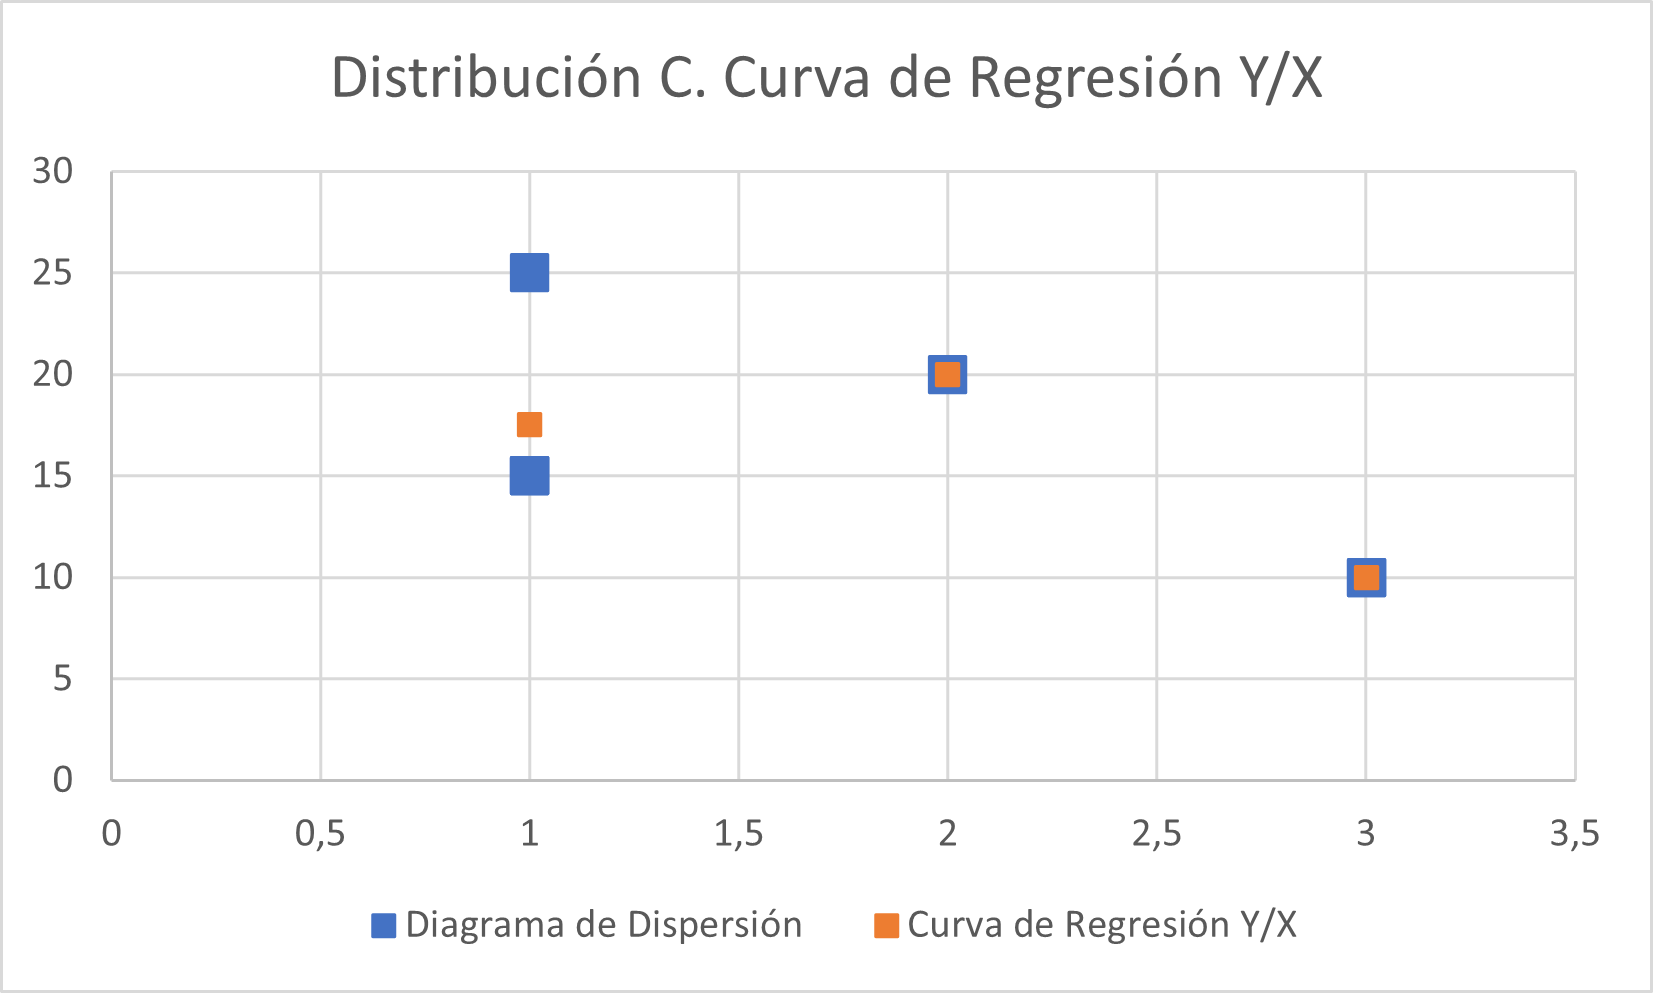
\includegraphics[width=0.6\linewidth]{Imagenes/Ej7.2.C.2.png}
                \caption{Curva de Regresión $Y/X$ de la distribución C.}
                \label{fig:Ej7.2.C.2}
            \end{figure}
        \end{enumerate}

        Podemos ver que, en los casos en los que hay dependencia funcional, la nube de puntos se superpone con la curva de regresión. Además, en el caso de la dependencia funcional recíproca, la curva de regresión de $Y/X$ coincide con la curva de regresión de $X/Y$.
    \end{enumerate}
\end{ejercicio}


\begin{ejercicio}
    De una muestra de 24 puestos de venta en un mercado de abastos se ha recogido información sobre el número de balanzas $(X)$ y el número de dependientes $(Y)$. Los resultados aparecen en la siguiente tabla:
    \begin{equation*}
        \begin{array}{c|cccc|c}
            X\backslash Y & 1 & 2 & 3 & 4 & n_{i.}\\ \hline
            1 & 1 & 2 & 0 & 0 & 3\\
            2 & 1 & 2 & 3 & 1 & 7\\
            3 & 0 & 1 & 2 & 6 & 9\\
            4 & 0 & 0 & 2 & 3 & 5\\ \hline
            n_{.j} & 2 & 5 & 7 & 10 & 24
        \end{array}
    \end{equation*}
    \begin{enumerate}
        \item Determinar las rectas de regresión.
        
        Sea el número de balanzas en un puesto de venta de un mercado, $X$; y el número de dependientes en dicho puesto de venta, $Y$ dos variables estadísticas con población $n=24$ y modalidades $x_1,\dots,x_4$ e $y_1,\dots, y_4$ respectivamente, con \emph{distribución de frecuencias}:
            $$\{(x_i,y_j),n_{ij}\}_{\substack{i=1,\dots,4\\j=1,\dots,4}}$$

        Para calcular el coeficiente de regresión lineal, antes son necesarios algunos cálculos:
        \begin{equation*}
            \bar{x} = \frac{1}{n}\sum_{i=0}^4 x_in_{i.} = \frac{64}{24} = 2.\bar{6}
            \qquad
            \bar{y} = \frac{1}{n}\sum_{j=0}^4 y_jn_{.j} = \frac{73}{24} = 3.041\bar{6}
        \end{equation*}
        \begin{equation*}
            \sigma_x^2 = \frac{1}{n}\sum_{i=0}^4 n_{i.}x_i^2 - \bar{x}^2
            = \frac{192}{24} - \bar{x}^2 = 0.\bar{8}
        \end{equation*}
        \begin{equation*}
            \sigma_y^2 = \frac{1}{n}\sum_{j=0}^4 n_{.j}y_j^2 - \bar{y}^2
            = \frac{245}{24} - \bar{y}^2 = 0.9566
        \end{equation*}
        \begin{equation*}
            \sigma_{xy} = \frac{1}{n}\sum_{i,j=0}^n n_{ij}x_iy_j - \bar{x}\bar{y} = \frac{209}{24} - \bar{x}\bar{y} = 0.597\bar{2}
        \end{equation*}
        Por tanto, la recta de regresión de $Y$ sobre $X$ es:
        \begin{equation*}
            y-\bar{y} = \frac{\sigma_{xy}}{\sigma_x^2}(x-\bar{x}) \Longrightarrow
            y = 0.6719x +1.25
        \end{equation*}
        La recta de regresión de $X$ sobre $Y$ es:
        \begin{equation*}
            x-\bar{x} = \frac{\sigma_{xy}}{\sigma_y^2}(y-\bar{y}) \Longrightarrow
            x = 0.6243y +0.7677
        \end{equation*}
    
        \item ¿Es apropiado suponer que existe una relación lineal entre las variables?\\

        Para ver cómo de bueno es el ajuste, usamos el coeficiente de determinación.
        \begin{equation*}
            r^2 = \frac{\sigma_{xy}^2}{\sigma_x^2 \sigma_y^2} = 0.4195
        \end{equation*}

        Además, vemos el coeficiente de correlación lineal:
        \begin{equation*}
            r = +\sqrt{r} = 0.64766
        \end{equation*}

        Como $r^2$ dista de $1$, no es un buen ajuste. En concreto, se explican el $41.92\%$ de los casos, menos de la mitad. Además, como $r$ también dista de $1$, podemos ver que no hay una correlación lineal alta entre ambas variables. 
    
        \item Predecir, a partir de los resultados, el número de balanzas que puede esperarse en un puesto con seis dependientes. ¿Es fiable esta predicción?
        
        Como se da una nueva modalidad de la variable $Y$, usamos la recta de regresión de $X$ sobre $Y$:
        \begin{equation*}
            x = 0.6243y +0.7677 = 0.6243(6) +0.7677 = 4.5135
        \end{equation*}
        Por tanto, se predice que habrá entre 4 y 5 balanzas. No obstante, como se ha razonado en el apartado anterior, esta predicción no es muy fiable.
    \end{enumerate}
\end{ejercicio}

\begin{ejercicio}
    Se eligen 50 matrimonios al azar y se les pregunta la edad de ambos al contraer matrimonio. Los resultados se recogen en la siguiente tabla, en la que $X$ denota la edad del hombre e $Y$ la de la mujer:
    \begin{equation*}
        \begin{array}{c||c|ccccc|c}
            X\backslash Y & c_i^x & (10, 20] & (20, 25] & (25, 30] & (30, 35] & (35, 40] & n_{i.}\\ \hline \hline
            c_j^y & & 15 & 22.5 & 27.5 & 32.5 & 37.5 &  \\ \hline
            (15, 18] & 16.5&  3 & 2 & 3 & 0 & 0 & 8\\
            (18, 21] & 19.5 & 0 & 4 & 2 & 2 & 0 & 8\\
            (21, 24] & 22.5 &  0 & 7 & 10 & 6 & 1 & 24\\
            (24, 27] & 25.5 &  0 & 0 & 2 & 5 & 3 & 10\\ \hline
            n_{.j} & & 3 & 13 & 17 & 13 & 4 & 50
        \end{array}
    \end{equation*}
    Estudiar la interdependencia lineal entre ambas variables.\\

    Sea la edad a la que el hombre contrajo matrimonio, $X$; y la edad a la que la mujer contrajo matrimonio, $Y$; dos variables estadísticas con población $n=50$ y modalidades $I^x_1, \dots, I^x_3$ e $I^y_1, \dots, I^y_3$ respectivamente, con \emph{distribución de frecuencias}:
        $$\left\{ (I^x_i,I^x_j), n_{ij}\right\}_{\substack{i=1,\dots,4\\j=1,\dots,5}}$$

    Para estudiar la interdependencia lineal, es necesario calcular el coeficiente de correlación lineal:
    \begin{equation*}
        r = \pm \sqrt{r^2} = \frac{\sigma_{xy}}{\sigma_x \sigma_y}
    \end{equation*}
    Calculamos por tanto los valores necesarios:
    \begin{equation*}
        \bar{x} = \frac{1}{n}\sum_{i=0}^4 c_i^x n_{i.} = \frac{1083}{50} = 21.66
        \qquad
        \bar{y} = \frac{1}{n}\sum_{j=0}^5 c_j^y n_{.j} = \frac{1377.5}{50} = 27.55
    \end{equation*}
    \begin{equation*}
        \sigma_x = \sqrt{\frac{1}{n}\sum_{i=0}^4 n_{i.} (c_i^x)^2 - \bar{x}^2}
        = \sqrt{\frac{23872.5}{50} - \bar{x}^2}
        = \sqrt{8.2944} = 2.88
    \end{equation*}
    \begin{equation*}
        \sigma_y = \sqrt{\frac{1}{n}\sum_{j=0}^5 n_{.j} (c_j^y)^2 - \bar{y}^2}
        = \sqrt{\frac{39468.75}{50} - \bar{y}^2}
        = \sqrt{30.3725} = 5.5111
    \end{equation*}
    \begin{equation*}
        \sigma_{xy} = \frac{1}{n} \sum_{i=0}^4 \sum_{j=0}^5 n_{ij}c_i^x c_j^y - \bar{x}\bar{y} = \frac{30318.75}{50} - \bar{x}\bar{y} = 9.642
    \end{equation*}

    Por tanto, tenemos que
    \begin{equation*}
        r = \frac{\sigma_{xy}}{\sigma_x \sigma_y} = 0.6075
    \end{equation*}

    De este resultado, obtenemos que la correlación es positiva. Además, la interdependencia lineal no es muy alta, ya que el valor de $r$ no es muy cercano al $1$. Por tanto, el nivel de correlación no termina de ser muy alto, sino que es más bien intermedio.
    
    Además, el ajuste lineal no es adecuado, ya que $r^2 = 0.3690$, y este es más cercano al $0$ que al $1$. De hecho, solo se predicen el $36.9\%$ de los valores.
\end{ejercicio}

\begin{ejercicio}
    Calcular el coeficiente de correlación lineal de dos variables cuyas rectas de regresión son:
    
    \begin{enumerate}
        \item $x+4y=1$
        \item $x+5y=2$
    \end{enumerate}

    Sean $X$ e $Y$ dos variables estadísticas con población $n$ y modalidades $x_1,\dots,x_k$ e $y_1,\dots,y_p$ respectivamente, con distribución de frecuencias absolutas
    $$\{(x_i,y_j);n_{ij}\}_{\substack{i=1,\dots,k\\j=1,\dots,p}}$$

    Supongamos que la primera recta es la recta de regresión de $Y/X$, mientras que la segunda es la recta de regresión de $X/Y$. Posteriormente comprobaremos si esta suposición es correcta.

    Como la primera recta es la recta de regresión de $Y/X$:
    \begin{equation*}
        y=-\frac{1}{4}x + \frac{1}{4} = \frac{\sigma_{xy}}{\sigma_x^2}x -\frac{\sigma_{xy}}{\sigma_x^2}\bar{x} + \bar{y}
    \end{equation*}
    Por tanto,
    \begin{equation*}
        -\frac{1}{4} = \frac{\sigma_{xy}}{\sigma_x^2} \qquad \frac{1}{4}=-\frac{\sigma_{xy}}{\sigma_x^2}\bar{x} + \bar{y} = \frac{1}{4}\bar{x} + \bar{y}
    \end{equation*}

    Como la segunda recta es la recta de regresión de $X/Y$:
    \begin{equation*}
        x=-5y+2 = \frac{\sigma_{xy}}{\sigma_y^2}x -\frac{\sigma_{xy}}{\sigma_y^2}\bar{y} + \bar{x}
    \end{equation*}
    Por tanto,
    \begin{equation*}
       -5 = \frac{\sigma_{xy}}{\sigma_y^2} \qquad 2=-\frac{\sigma_{xy}}{\sigma_y^2}\bar{y} + \bar{x} = 5\bar{y} + \bar{x}
    \end{equation*}

    El coeficiente de determinación lineal es, por tanto:
    \begin{equation*}
        r^2 = \frac{\sigma_{xy}}{\sigma_x^2} \cdot \frac{\sigma_{xy}}{\sigma_y^2} = -\frac{1}{4}\cdot (-5) = \frac{5}{4}
    \end{equation*}
    Como $0\leq r^2 \leq 1$, deducimos que esta suposición \textbf{no} es correcta. Por tanto, sabemos que la primera recta es la recta de regresión de $X/Y$, mientras que la segunda es la recta de regresión de $Y/X$.
    
    Como la primera recta es la recta de regresión de $X/Y$:
    \begin{equation*}
       x=-4y+1 = \frac{\sigma_{xy}}{\sigma_y^2}y -\frac{\sigma_{xy}}{\sigma_y^2}\bar{y} + \bar{x}
    \end{equation*}
    Por tanto,
    \begin{equation*}
        -4 = \frac{\sigma_{xy}}{\sigma_y^2} \qquad 1=-\frac{\sigma_{xy}}{\sigma_y^2}\bar{y} + \bar{x} = 4\bar{y} + \bar{x}
    \end{equation*}

    Como la segunda recta es la recta de regresión de $Y/X$:
    \begin{equation*}
        y=-\frac{1}{5}x+\frac{2}{5} = \frac{\sigma_{xy}}{\sigma_x^2}x -\frac{\sigma_{xy}}{\sigma_x^2}\bar{x} + \bar{y}
    \end{equation*}
    Por tanto,
    \begin{equation*}
       -\frac{1}{5} = \frac{\sigma_{xy}}{\sigma_x^2} \qquad \frac{2}{5}=-\frac{\sigma_{xy}}{\sigma_x^2}\bar{x} + \bar{y} = \frac{1}{5}\bar{x} + \bar{y}
    \end{equation*}

    El coeficiente de determinación lineal es, por tanto:
    \begin{equation*}
        r^2 = \frac{\sigma_{xy}}{\sigma_x^2} \cdot \frac{\sigma_{xy}}{\sigma_y^2} = -\frac{1}{5}\cdot (-4) = \frac{4}{5}
    \end{equation*}
    Como $0\leq r^2 \leq 1$, deducimos que esta suposición \textbf{sí} es la correcta.

    Por tanto, como se pide el coeficiente de regresión lineal, tenemos que:
    \begin{equation*}
        r = -\sqrt{r^2} = -0.8944
    \end{equation*}
    donde es necesario que hemos tomado la raíz con signo negativo, ya que la covarianza, que determina el signo del coeficiente de regresión lineal,  tiene signo negativo.
\end{ejercicio}

\begin{ejercicio}
    Consideremos una distribución bidimensional en la que la recta de regresión de $Y$ sobre $X$ es $y = 5x - 20$, y $\sum y_j^2 n_{\cdot j} = 3240$. Supongamos, además, que la distribución marginal de $X$ es:
    \begin{equation*}
        \begin{array}{c|cccc}
            x_i & 3 & 5 & 8 & 9 \\ \hline
            n_{i\cdot} & 5 & 1 & 2 & 1 
        \end{array}
    \end{equation*}
    Determinar la recta de regresión de $X$ sobre $Y$, y la bondad de los ajustes lineales.\\

    Sean $X$ y $Y$ dos variables estadísticas con población $n=9$ y modalidades $x_1, \dots, x_4$ e $y_1, \dots, y_p$ respectivamente, con \emph{distribución de frecuencias}:
        $$\left\{ (x_i,y_j), n_{ij}\right\}_{\substack{i=1,\dots,4\\j=1,\dots,p}}$$

    De la distribución marginal de $X$, obtengo directamente los siguientes dos resultados:
    \begin{equation*}
        \bar{x} = \frac{1}{n}\sum_{i=0}^4 n_{i.}x_i = \frac{45}{9} = 5
    \end{equation*}
    \begin{equation*}
        \sigma_x^2 = \frac{1}{n}\sum_{i=0}^4 n_{i.}x_i^2 - \bar{x}^2 = \frac{279}{9} - \bar{x}^2 = 6
    \end{equation*}

    La ecuación de la recta de regresión de $Y$ sobre $X$ es:
    \begin{equation*}
        y=ax+b = \frac{\sigma_{xy}}{\sigma_x^2}x -\frac{\sigma_{xy}}{\sigma_x^2} \bar{x} + \bar{y} = 5x-20
    \end{equation*}

    Igualando términos:
    \begin{equation*}
        a = \frac{\sigma_{xy}}{\sigma_x^2} = 5 \Longrightarrow \sigma_{xy} = 5 \cdot {\sigma_x^2} = 30
    \end{equation*}
    \begin{equation*}
        b = -\frac{\sigma_{xy}}{\sigma_x^2} \bar{x} + \bar{y} = -20 \Longrightarrow \bar{y} = -20 + \frac{\sigma_{xy}}{\sigma_x^2} \bar{x} = -20+5\bar{x} = 5
    \end{equation*}

    Teniendo $\bar{y}$ y usando la información dada por el enunciado, calculamos la varianza de la variable $Y$:
    \begin{equation*}
        \sigma_y^2 = \frac{1}{n}\sum_{j=0}^p y_j^2 n_{.j} - \bar{y}^2 = \frac{3240}{9} - \bar{y}^2 = 335
    \end{equation*}

    Por tanto, calculamos la recta de regresión de $X$ sobre $Y$:
    \begin{equation*}
        x-\bar{x} = \frac{\sigma_{xy}}{\sigma_y^2} (y-\bar{y}) \Longrightarrow x=0.08955y+4.5522
    \end{equation*}

    Para hallar la bondad de los ajustes lineales, calculo el coeficiente de determinación lineal.
    \begin{equation*}
        \eta_{X/Y}^2 = \eta_{Y/X}^2 = r^2 = \frac{\sigma_{xy}^2}{\sigma_x \sigma_y} = 0.4478
    \end{equation*}

    Como $r^2$ es más cercano a 0 que al 1, entonces explica menos de la mitad de los datos. Por tanto, suponer una relación lineal no es lo ideal.

    Además, el coeficiente de correlación lineal es $r=+\sqrt{r^2} = 0.6692$. Como no es muy cercano a 1, la interdependencia lineal entre ambas variables no es muy alta.
\end{ejercicio}

\begin{ejercicio}
    De las estadísticas de ``Tiempos de vuelo y consumos de combustible'' de una compañía aérea, se han obtenido datos relativos a 24 trayectos distintos realizados por el avión DC-9. A partir de estos datos se han obtenido las siguientes medidas:
    $$\sum y_i = 219.719\qquad \sum y_i^2= 2396.504 \qquad \sum x_iy_i = 349.486$$
    $$\sum x_i = 31.470 \qquad \sum x_i^2 = 51.075 \qquad \sum x_i^2y_i = 633.993$$
    $$\sum x_i^4 = 182.977 \qquad \sum x_i^3 = 93.6$$

    La variable $Y$ expresa el consumo total de combustible, en miles de libras, correspondiente a un vuelo de duración $X$ (el tiempo se expresa en horas, y se utilizan como unidades de orden inferior fracciones decimales de la hora).
    \begin{enumerate}
        \item\label{Ej12:Ap.1} Ajustar un modelo del tipo $Y = aX+b$. ¿Qué consumo total se estimará para un programa de vuelos compuesto de 100 vuelos de media hora, 200 de una hora y 100 de dos horas? ¿Es fiable esta estimación?

        Sea la duración del vuelo, $X$, en horas; y el consumo de combustible, $Y$, en miles de libras; dos variables estadísticas con población $n=24$ y modalidades $x_1, \dots, x_{24}$ e $y_1, \dots, y_{24}$ respectivamente, con \emph{distribución de frecuencias}:
        $$\left\{ (x_i,y_j), n_{ij}\right\}_{\substack{i=1,\dots,24\\j=1,\dots,24}}$$

        Como son vuelos distintos, supongo las siguientes frecuencias:
        \begin{equation*}
            n_{ij} = \delta_{ij} = \left\{
            \begin{array}{ccc}
                1 & si & i=j \\
                0 & si & i\neq j
            \end{array}
            \right.
        \end{equation*}

        Para calcular la recta de regresión de $Y$ sobre $X$, calculo previamente algunos datos.
        \begin{equation*}
            \bar{x} = \frac{1}{n} \sum_{i=1}^{24} n_{i.}x_i = \frac{1}{24} \sum x_i = 1.31125
            \qquad
            \bar{y} = \frac{1}{n} \sum_{j=1}^{24} n_{.j}y_j = \frac{1}{24} \sum y_i = 9.15496
        \end{equation*}
        \begin{equation*}
            \sigma_{xy} = \frac{1}{n}\sum_{i=0}^{24} x_iy_in_{ii} -\bar{x}\bar{y} = \frac{1}{24}\sum x_iy_i -\bar{x}\bar{y} = 2.557475
        \end{equation*}
        \begin{equation*}
            \sigma_x^2 = \frac{1}{n} \sum_{i=1}^{24} n_{i.}x_i^2 -\bar{x}^2 = \frac{1}{24} \sum x_i^2 -\bar{x}^2 = 0.40875
        \end{equation*}
        \begin{equation*}
            \sigma_y^2 = \frac{1}{n} \sum_{j=1}^{24} n_{.j}y_j^2 -\bar{y}^2 = \frac{1}{24} \sum y_i^2 -\bar{y}^2 = 16.04104
        \end{equation*}
        Por tanto, la recta de regresión de $Y$ sobre $X$ es:
        \begin{equation*}
            y-\bar{y} = \frac{\sigma_{xy}}{\sigma_x^2} (x-\bar{x}) \Longrightarrow
            y = 6.25682x +0.9507
        \end{equation*}

        Para ver la bondad del ajuste lineal, estudio $r^2$:
        \begin{equation*}
            r^2 = \frac{\sigma_{xy}^2}{\sigma_x^2 \sigma_y^2} = 0.997545
        \end{equation*}
        
        Estimamos ahora para el programa de vuelos pedido.
        \begin{itemize}
            \item Para un vuelo de media hora, tenemos un consumo de:
            \begin{equation*}
                y = 6.25682x +0.9507 = 6.25682\cdot 0.5 +0.9507 = 4.07911 \text{ miles de libras.}
            \end{equation*}

            \item Para un vuelo de una hora, tenemos consumo de:
            \begin{equation*}
                y = 6.25682x +0.9507 = 6.25682\cdot 1 +0.9507 = 7.20752 \text{ miles de libras.}
            \end{equation*}

            \item Para un vuelo de dos horas, tenemos un consumo de:
            \begin{equation*}
                y = 6.25682x +0.9507 = 6.25682\cdot 2 +0.9507 = 13.46434 \text{ miles de libras.}
            \end{equation*}
        \end{itemize}
        Por tanto, para el programa total de vuelos pedido, el consumo será de:
        \begin{equation*}
            y_T = 100\cdot 4.07911 + 200\cdot 7.20752 + 100\cdot 13.46434 = 3195.849\text{ miles de libras.}
        \end{equation*}

        Como $r^2=0.997545\approx 1$, vemos que es un ajuste de buena calidad y, por tanto, es una estimación muy fiable.

        \item Ajustar un modelo del tipo $Y = a + bX + cX^2.$ ¿Qué consumo total se estimará para el mismo programa de vuelos del apartado $a)$?
        
        Para encontrar los parámetros $a,b,c$ mediante el ajuste de mínimos cuadrados, hemos de resolver el siguiente sistema de ecuaciones ortonormales:
        \begin{equation*}
            \left\{ \begin{array}{rcrcrcr}
                m_{01} &=& a &+&bm_{10} &+& cm_{20}  \\
                m_{11} &=& am_{10} &+& bm_{20} &+&cm_{30}  \\
                m_{21} &=& am_{20} &+& bm_{30} &+&cm_{40}  \\
            \end{array}\right.
        \end{equation*}

        equivalentemente, y usando la definición de los momentos conjuntos respecto al origen, tenemos que el sistema de ecuaciones ortonormales es:
        \begin{equation*}
            \left\{ \begin{array}{rcrcrcr}
                \bar{y} &=& a &+&b\bar{x} &+& cm_{20}  \\
                m_{11} &=& a\bar{x} &+& bm_{20} &+&cm_{30}  \\
                m_{21} &=& am_{20} &+& bm_{30} &+&cm_{40}  \\
            \end{array}\right.
        \end{equation*}

        Calculo por tanto los momentos que faltan:
        \begin{equation*}
            m_{30} = \frac{1}{n}\sum_{i,j=1}^{24} n_{ij}x_i^3 y_j^0 = \frac{1}{24} \sum x_i^3 = 3.9
            \qquad
            m_{40} = \frac{1}{n}\sum_{i,j=1}^{24} n_{ij}x_i^4 y_j^0 = \frac{1}{24} \sum x_i^4 = 7.62404
        \end{equation*}
        \begin{equation*}
            m_{20} = \frac{1}{n}\sum_{i,j=1}^{24} n_{ij}x_i^2 y_j^0 = \frac{1}{24} \sum x_i^2 = \frac{51.075}{0.24} = 2.1281
        \end{equation*}
        \begin{equation*}
            m_{11} = \frac{1}{n}\sum_{i,j=1}^{24} n_{ij}x_i^1 y_j^1 = \frac{1}{24} \sum x_iy_i = \frac{349.486}{24} = 14.5619
        \end{equation*}
        \begin{equation*}
            m_{21} = \frac{1}{n}\sum_{i,j=1}^{24} n_{ij}x_i^2 y_j^1 = \frac{1}{24} \sum x_i^2 y_i = 26.416375
        \end{equation*}

        Por tanto, el sistema queda:
        \begin{equation*}
            \left\{ \begin{array}{rcrcrcr}
                9.15496 &=& a &+&1.31125 b &+& 2.1281  c  \\
                14.5619&=& 1.31125a &+& 2.1281 b &+&3.9 c  \\
                26.416375 &=& 2.1281 a &+& 3.9 b &+&7.62404 c  \\
            \end{array}\right.
        \end{equation*}
        
        Resolviendo, obtenemos que
        \begin{equation*}
            a=0.79855\qquad b=6.54482 \qquad c=-0.10596
        \end{equation*}

        Por tanto, tenemos que la parábola de regresión de $Y$ sobre $X$ es:
        \begin{equation*}
            y=0.79855 + 6.54482x -0.10596x^2
        \end{equation*}

        Estimamos ahora para el programa de vuelos pedido.
        \begin{itemize}
            \item Para un vuelo de media hora, tenemos un consumo de:
            \begin{equation*}
                y = 0.79855 + 6.54482\cdot(0.5) -0.10596\cdot(0.5)^2 = 4.04447 \text{ miles de libras.}
            \end{equation*}

            \item Para un vuelo de una hora, tenemos consumo de:
            \begin{equation*}
                y = 6.25682x +0.9507 = 6.25682\cdot 1 +0.9507 = 7.23741 \text{ miles de libras.}
            \end{equation*}

            \item Para un vuelo de dos horas, tenemos un consumo de:
            \begin{equation*}
                y = 6.25682x +0.9507 = 6.25682\cdot 2 +0.9507 = 13.46435 \text{ miles de libras.}
            \end{equation*}
        \end{itemize}
        Por tanto, para el programa total de vuelos pedido, el consumo será de:
        \begin{equation*}
            y_T = 100\cdot 4.04447 + 200\cdot 7.23741 + 100\cdot 13.46435 = 3198.364\text{ miles de libras.}
        \end{equation*}

        \item ¿Cuál de los dos modelos se ajusta mejor? Razonar la respuesta.\\
        Ambos ajustes tienen el mismo coeficiente de determinación, por lo que se podría pensar en un primer momento que ambos son iguales. No obstante, al haber una tercera ecuación (ser de grado 2), incluye un tercer parámetro y entonces añade información. Por tanto, el ajuste parabólico se ajusta mejor\footnote{En el caso de tener las distintas modalidades, podríamos calcular $\sigma_{ey}^2$ para cada ajuste y veríamos que, en el caso de la parábola, es mayor.}.

        No obstante, podemos ver que las diferencias son insignificantes, ya que las predicciones están muy próximas debido al alto valor de $r^2$.
    \end{enumerate}
\end{ejercicio}

\begin{ejercicio}
    La curva de Engel, que expresa el gasto en un determinado bien en función de la renta, adopta en ocasiones la forma de una hipérbola equilátera. Ajustar dicha curva a los siguientes datos, en los que $X$ denota la renta en miles de euros e $Y$ el gasto en euros. Cuantificar la bondad del ajuste:
    \begin{equation*}
        \begin{array}{c|cccc}
            X & 10 & 12.5 & 20 & 25\\ \hline
            Y & 50 & 90 & 160 & 180 \\ \hline \hline
            Z & 0.1 & 0.08 & 0.05 & 0.04
        \end{array}
    \end{equation*}

    Sea la renta, $X$, en miles de euros; y el gasto en determinado bien, $Y$, en euros; dos variables estadísticas con población $n=4$ y modalidades $x_1, \dots, x_4$ e $y_1, \dots, y_4$ respectivamente, con \emph{distribución de frecuencias}:
        $$\left\{ (x_i,y_j), n_{ij}\right\}_{\substack{i=1,\dots,4\\j=1,\dots,4}}$$

    Como el ajuste es de la forma $y=\frac{a}{x}+b$, realizo el cambio de variable $z=\frac{1}{x}$. Por tanto, calculo la recta de regresión de $Y$ sobre $Z$.

    Para calcular el coeficiente de regresión de $Y$ sobre $Z$, necesito calcular antes varios datos:
    \begin{equation*}
        \bar{z} = \frac{1}{n}\sum_{i=0}^4 n_{i.}z_i = \frac{0.27}{4} = 0.0675
        \qquad
        \bar{y} = \frac{1}{n}\sum_{j=0}^4 n_{.j}y_j = \frac{480}{4} = 120
    \end{equation*}
    \begin{equation*}
        \sigma_{zy} = \frac{1}{n} \sum_{i,j=0}^4 n_{ij}z_iy_j -\bar{z}\bar{y}
        = \frac{1}{n} \sum_{i,j=0}^4 n_{ij}\frac{y_j}{x_i} -\bar{z}\bar{y}
        =  \frac{27.4}{4} -\bar{z}\bar{y} = -1.25
    \end{equation*}
    \begin{equation*}
        \sigma_z^2 = \frac{1}{n}\sum_{i=0}^4 n_{i.}z_i^2 - \bar{z}^2
        = \frac{1}{n}\sum_{i=0}^4 \frac{1}{x_i^2} - \bar{z}^2
        = \frac{0.0205}{4} - \bar{z}^2 = 5.6875\cdot 10^{-4}
    \end{equation*}
    \begin{equation*}
        \sigma_y^2 = \frac{1}{n}\sum_{j=0}^4 n_{.j}y_j^2 - \bar{y}^2
        = \frac{68600}{4} - \bar{y}^2 = 2750
    \end{equation*}

    Por tanto, la recta de regresión de $Y$ sobre $Z$ es:
    \begin{equation*}
        y-\bar{y} = \frac{\sigma_{zy}}{\sigma_z^2}(z-\bar{z}) \Longrightarrow y = -2197.8022z+268.3516
    \end{equation*}

    Deshaciendo el cambio de variable, obtengo la curva de regresión hiperbólica de $Y$ sobre $X$:
    \begin{equation*}
        y = -\frac{2197.8022}{x}+268.3516
    \end{equation*}

    Para estudiar la bondad del ajuste hiperbólico, necesitamos interpretar el coeficiente de determinación.
    \begin{equation*}
        r^2 = \frac{\sigma_{zy}^2}{\sigma_z^2 \sigma_y^2} = 0.999
    \end{equation*}

    Por tanto, este ajusta el $99.9\%$ de los casos, por lo que el ajuste es prácticamente ideal, ya que $r^2\approx 1$.
\end{ejercicio}

\begin{ejercicio}\label{ej:2.Ejercicio14}
    Se dispone de la siguiente información referente al gasto en espectáculos ($Y$, en euros) y la renta disponible mensual ($X$, en cientos de euros) de 6 familias:
    \begin{equation*}
        \begin{array}{c|cccccc}
            Y & 30 & 50 & 70 & 80 & 120 & 140 \\ \hline
            X & 9 & 10 & 12 & 15 & 22 & 32
        \end{array}
    \end{equation*}
    Explicar el comportamiento de $Y$ por $X$ mediante:
    \begin{enumerate}
        \item Relación lineal.\label{Ej:Ej14.Ap_A}

        Sea la renta disponible mensual, $X$, en cientos de euros; y el gasto en espectáculos, $Y$, en euros; dos variables estadísticas con población $n=6$ y modalidades $x_1, \dots, x_6$ e $y_1, \dots, y_6$ respectivamente, con \emph{distribución de frecuencias}:
        $$\left\{ (x_i,y_j), n_{ij}\right\}_{\substack{i=1,\dots,6\\j=1,\dots,6}}$$

        Para calcular la recta de regresión, hemos de hallar en primer lugar otros datos.
        \begin{equation*}
            \bar{x} = \frac{1}{n}\sum_{i=0}^6 x_{i}n_{i.} = \frac{100}{6} = 16.\bar{6}
            \qquad
            \bar{y} = \frac{1}{n}\sum_{j=0}^6 y_{j}n_{.j} = \frac{490}{6} = 81.\bar{6}
        \end{equation*}
        \begin{equation*}
            \sigma_{xy} = \frac{1}{n}\sum_{i,j=0}^6 x_iy_j n_{ij} - \bar{x}\bar{y} = \frac{9930}{6} - \bar{x}\bar{y} = 293.\bar{8}
        \end{equation*}
        \begin{equation*}
            \sigma_x^2 = \frac{1}{n}\sum_{i=0}^6 n_{ij}x_i^2 - \bar{x}^2 = \frac{2058}{6} - \bar{x}^2 = 65.\bar{2}
        \end{equation*}
        \begin{equation*}
            \sigma_y^2 = \frac{1}{n}\sum_{j=0}^6 n_{ij}y_j^2 - \bar{y}^2 = \frac{48700}{6} - \bar{y}^2 = 1447.\bar{2}
        \end{equation*}

        Por tanto, recta de regresión de $Y$ sobre $X$ es:
        \begin{equation*}
            y-\bar{y} = \frac{\sigma_{xy}}{\sigma_x^2}(x-\bar{x}) \Longrightarrow y=4.5059x +6.56729
        \end{equation*}
        
        Vara ver si es correcto el ajuste o no, calculamos el coeficiente de determinación:
        \begin{equation*}
            \eta_{Y/X}^2 = \frac{\sigma_{ey}^2}{\sigma_y^2} = r^2 = \frac{\sigma_{xy}^2}{\sigma_x^2 \sigma_y^2} = 0.91503
        \end{equation*}

        La varianza residual, al ser el ajuste lineal en los parámetros, queda:
        \begin{equation*}
            \sigma_{ry}^2 = (1-r^2)\sigma_y^2 = 122.97
        \end{equation*}

        Estos resultados los podemos ver en el diagrama de dispersión de la figura \ref{fig:Ed14.a}.
        \begin{figure}[H]
            \centering
            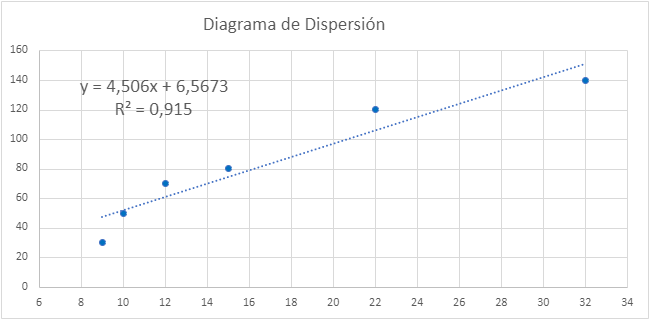
\includegraphics[width=0.6\linewidth]{Imagenes/Ej14.a.png}
            \caption{Diagrama de dispersión del ejercicio \ref{ej:2.Ejercicio14}.\ref{Ej:Ej14.Ap_A}}
            \label{fig:Ed14.a}
        \end{figure}
        
        \item Hipérbola equilátera. \label{Ej:Ej14.Ap_B}

        Como la recta será de la forma $ y=\frac{a}{x}+b$, es necesario realizar en primer lugar el cambio de variable $z=\frac{1}{x}$. Queda por tanto de la siguiente manera:
        \begin{equation*}
            \begin{array}{c|cccccc}
                Y & 30 & 50 & 70 & 80 & 120 & 140 \\ \hline
                Z & 0.\bar{1} & 0.1 & 0.08\bar{3} & 0.0\bar{6} & 0.0\overline{45} & 0.03125 \\ \hline \hline
                X & 9 & 10 & 12 & 15 & 22 & 32
            \end{array}
        \end{equation*}
        Por tanto, calculamos la recta de regresión de $Y$ sobre $Z$:
        \begin{equation*}
            \bar{z} = \frac{1}{n}\sum_{i=0}^6 z_{i}n_{i.} = \frac{0.4378}{6} = 0.073
            \qquad
            \bar{y} = \frac{1}{n}\sum_{j=0}^6 y_{j}n_{.j} = \frac{490}{6} = 81.\bar{6}
        \end{equation*}
        \begin{equation*}
            \sigma_{zy} = \frac{1}{n}\sum_{i,j=0}^6 z_iy_j n_{ij} - \bar{z}\bar{y} = \frac{29.3295}{6} - \bar{x}\bar{y} = -1.0734
        \end{equation*}
        \begin{equation*}
            \sigma_z^2 = \frac{1}{n}\sum_{i=0}^6 n_{ij}z_i^2 - \bar{z}^2 = \frac{0.036777}{6} - \bar{z}^2 = 8.00541\cdot 10^{-4}
        \end{equation*}
        \begin{equation*}
            \sigma_y^2 = \frac{1}{n}\sum_{j=0}^6 n_{ij}y_j^2 - \bar{y}^2 = \frac{48700}{6} - \bar{y}^2 = 1447.\bar{2}
        \end{equation*}

        Por tanto, recta de regresión de $Y$ sobre $Z$ es:
        \begin{equation*}
            y-\bar{y} = \frac{\sigma_{zy}}{\sigma_z^2}(z-\bar{z}) \Longrightarrow y=-1340.843z +179.55
        \end{equation*}

        Deshaciendo el cambio de variable:
        \begin{equation*}
            y=-\frac{1340.843}{x} +179.55
        \end{equation*}
        
        Para ver si es correcto el ajuste o no, calculamos el coeficiente de determinación:
        \begin{equation*}
            r^2 = \frac{\sigma_{zy}^2}{\sigma_z^2 \sigma_y^2} = 0.98102
        \end{equation*}

        La varianza residual, al ser el ajuste lineal en los parámetros, queda:
        \begin{equation*}
            \sigma_{ry}^2 = (1-r^2)\sigma_y^2 = 27.46
        \end{equation*}
        
        \item Curva potencial. \label{Ej:Ej14.Ap_C}
        
        Como la curva será de la forma $y=bx^a$, es necesario realizar en primer lugar un cambio de variable. Para ello, aplico el $\ln$ y establecemos $y'=\ln y$, $b'=\ln b$, $x'=\ln x$. Queda por tanto de la siguiente manera:
        \begin{equation*}
            \begin{array}{c|cccccc}
                Y & 30 & 50 & 70 & 80 & 120 & 140 \\ \hline
                X & 9 & 10 & 12 & 15 & 22 & 32 \\ \hline \hline
                Y' & 3.4012 & 3.912 & 4.2485 & 4.38203 & 4.7875 & 4.9416 \\ \hline
                X' & 2.197 & 2.3026 & 2.4849 & 2.7086 & 3.091 & 2.4849
            \end{array}
        \end{equation*}
        Por tanto, calculamos la recta de regresión de $Y'$ sobre $X'$:
        \begin{equation*}
            \bar{x'} = \frac{1}{n}\sum_{i=0}^6 x'_{i}n_{i.} =  \frac{1}{n}\sum_{i=0}^6 \ln (x_{i})n_{i.}=\frac{1}{n}\ln\left(\prod_{i=0}^6 x_i\right) = \frac{\ln 11404800}{6} = 2.70826
        \end{equation*}
        \begin{equation*}
            \bar{y'} = \frac{1}{n}\sum_{j=0}^6 y'_{j}n_{.j} =  \frac{1}{n}\sum_{j=0}^6 \ln (y_{j})n_{.j}=\frac{1}{n}\ln\left(\prod_{j=0}^6 y_j\right) = \frac{\ln 14112\cdot10^7}{6} = 4.2788
        \end{equation*}
        \begin{equation*}
            \sigma_{x'y'} =
            \frac{1}{n}\sum_{i,j=0}^6 x'_iy'_j n_{ij} - \bar{x'}\bar{y'} = \frac{70.8296}{6} - \bar{x'}\bar{y'} = 0.2168
        \end{equation*}        
        \begin{equation*}
            \sigma_{x'}^2
            = \frac{1}{n}\sum_{i=0}^6 n_{ij} (x_i')^2 - \bar{x'}^2
            = \frac{45.20386}{6} - \bar{x'}^2 = 0.1993
        \end{equation*}
        \begin{equation*}
            \sigma_{y'}^2 = \frac{1}{n}\sum_{j=0}^6 n_{ij}(y'_j)^2 - \bar{y'}^2 = \frac{111.4638}{6} - \bar{y'}^2 = 0.26918
        \end{equation*}

        Por tanto, recta de regresión de $Y'$ sobre $X'$ es:
        \begin{equation*}
            y'-\bar{y'} = \frac{\sigma_{x'y'}}{\sigma_{x'}^2}(x'-\bar{x'}) \Longrightarrow y'=1.0878x'+1.3327
        \end{equation*}

        Deshaciendo el cambio de variable:
        \begin{equation*}
            \ln y=1.0878\ln x +1.3327 \Longrightarrow y = e^{1.0878\ln x + 1.3327} = e^{1.3327}x^{1.0878} = 3.7914x^{1.0878}
        \end{equation*}
        \begin{equation*}
            y = 3.7914x^{1.0878}
        \end{equation*}
        
        Para estudiar la bondad del ajuste, calculamos la varianza residual teniendo en cuenta que el ajuste \textbf{no} es lineal en los parámetros:
        \begin{multline*}
            \sigma_{ry}^2 = \frac{1}{n} \sum_{i,j=1}^6 n_{ij} (y_j - f(x_i))^2
            =\\=
            \frac{(30-41.3833)^2 + (50-46.4087)^2 + (70-56.5891)^2}{6} +\\+ \frac{(80-72.1359)^2 +(120-109.4176)^2 +(140-164.4757)^2}{6}
            =\\=
            \frac{1095.2203}{6}=182.5367
        \end{multline*}
        

        Estos resultados los podemos ver en el diagrama de dispersión de la figura \ref{fig:Ed14.c}.
        \begin{figure}[H]
            \centering
            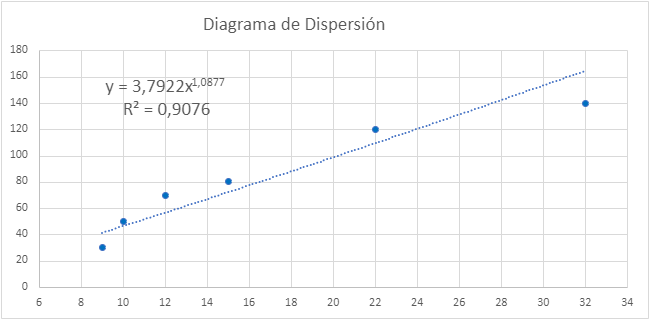
\includegraphics[width=0.6\linewidth]{Imagenes/Ej14.c.png}
            \caption{Diagrama de dispersión del ejercicio \ref{ej:2.Ejercicio14}.\ref{Ej:Ej14.Ap_C}}
            \label{fig:Ed14.c}
        \end{figure}
        
        \item Curva exponencial.\label{Ej:Ej14.Ap_D}

        Como la curva será de la forma $y=ba^{x}$, es necesario realizar en primer lugar un cambio de variable. Para ello, aplico el $\ln$ y establecemos $y'=\ln y$, $b'=\ln b$. El cambio de variable, por tanto, es:
        \begin{equation*}
            \ln y = \ln (ba^{x}) = \ln b + \ln(a)x \Longrightarrow y' = b'+a'x
        \end{equation*}
        Queda por tanto de la siguiente manera:
        \begin{equation*}
            \begin{array}{c|cccccc}
                Y & 30 & 50 & 70 & 80 & 120 & 140 \\ \hline
                X & 9 & 10 & 12 & 15 & 22 & 32 \\ \hline \hline
                Y' & 3.4012 & 3.912 & 4.2485 & 4.38203 & 4.7875 & 4.9416
            \end{array}
        \end{equation*}
        Por tanto, calculamos la recta de regresión de $Y'$ sobre $X$:
        \begin{equation*}
            \bar{x} = \frac{1}{n}\sum_{i=0}^6 x_{i}n_{i.} = \frac{100}{6} = 16.\bar{6}
        \end{equation*}
        \begin{equation*}
            \bar{y'} = \frac{1}{n}\sum_{j=0}^6 y'_{j}n_{.j} =  \frac{1}{n}\sum_{j=0}^6 \ln (y_{j})n_{.j}=\frac{1}{n}\ln\left(\prod_{j=0}^6 y_j\right) = \frac{\ln 14112\cdot10^7}{6} = 4.2788
        \end{equation*}
        \begin{equation*}\begin{split}
            \sigma_{xy'}
            &= \frac{1}{n}\sum_{i,j=0}^6 x_iy'_j n_{ij} - \bar{x}\bar{y'}
            = \frac{1}{n}\sum_{i,j=0}^6 x_i\ln y_j - \bar{x}\bar{y'}
            = \frac{1}{n}\sum_{i,j=0}^6 \ln (y_j^{x_i}) - \bar{x}\bar{y'} \\
            &= \frac{1}{n} \ln\left( \prod_{i,j=0}^6 y_j^{x_i} \right) - \bar{x}\bar{y'}
            = \frac{449.89945}{6} - \bar{x}\bar{y'} = 3.6699
        \end{split}\end{equation*}        
        \begin{equation*}
            \sigma_x^2 = \frac{1}{n}\sum_{i=0}^6 n_{ij}x_i^2 - \bar{x}^2 = \frac{2058}{6} - \bar{x}^2 = 65.\bar{2}
        \end{equation*}
        \begin{equation*}
            \sigma_{y'}^2 = \frac{1}{n}\sum_{j=0}^6 n_{ij}(y'_j)^2 - \bar{y'}^2 = \frac{111.4638}{6} - \bar{y'}^2 = 0.26918
        \end{equation*}

        Por tanto, recta de regresión de $Y'$ sobre $X$ es:
        \begin{equation*}
            y'-\bar{y'} = \frac{\sigma_{xy'}}{\sigma_{x}^2}(x-\bar{x}) \Longrightarrow y'=0.05627x +3.341
        \end{equation*}

        Deshaciendo el cambio de variable:
        \begin{equation*}
            \ln y=0.05627x +3.341 \Longrightarrow y = e^{0.05627x +3.341} = e^{3.341}e^{0.05627x} = 28.2475e^{0.05627x}
        \end{equation*}
        \begin{equation*}
            y = 28.2475e^{0.05627x} \Longrightarrow y = 28.2475\cdot 1.05788^x
        \end{equation*}
        
        Para estudiar la bondad del ajuste, calculamos la varianza residual teniendo en cuenta que el ajuste \textbf{no} es lineal en los parámetros:
        \begin{multline*}
            \sigma_{ry}^2 = \frac{1}{n} \sum_{i,j=1}^6 n_{ij} (y_j - f(x_i))^2
            =\\=
            \frac{(30-46.87137)^2 + (50-49.5843)^2 + (70-55.4903)^2}{6} +\\+ \frac{(80-65.69406)^2 +(120-97.4049)^2 +(140-170.9799)^2}{6}
            =\\=
            \frac{2170.2999}{6}=361.71667
        \end{multline*}
        

        Estos resultados los podemos ver en el diagrama de dispersión de la figura \ref{fig:Ed14.d}.
        \begin{figure}[H]
            \centering
            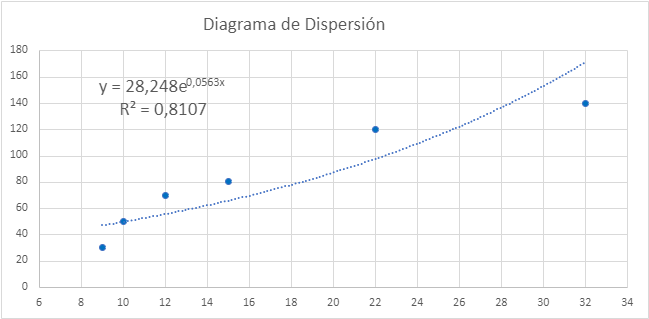
\includegraphics[width=0.6\linewidth]{Imagenes/Ej14.d.png}
            \caption{Diagrama de dispersión del ejercicio \ref{ej:2.Ejercicio14}.\ref{Ej:Ej14.Ap_D}}
            \label{fig:Ed14.d}
        \end{figure}
    \end{enumerate}
    
    ¿Qué ajuste es más adecuado?
    
    Como el menor valor de $\sigma_{ry}^2$ es para el ajuste hiperbólico, concluimos que este es el ajuste más adecuado, ya que deja sin explicar la menor cantidad de datos. En ese caso, vemos que $r^2=0.98102$, por lo que explica adecuadamente más del $98\%$ de los casos.
\end{ejercicio}
